\documentclass{simple-notes}
\usepackage{physics}
\usepackage{amsmath}
\usepackage{amssymb}
\usepackage[backend=bibtex, style=authoryear]{biblatex}
\addbibresource{Optimal_Pulse_Control.bib}
\title{GRAPE for Ion Trap System}
\author{Kun-Long Wu}
\newcommand{\closef}{\mathbf{F}}
\newcommand{\openf}{\mathcal{F}}
\newcommand{\dvbar}[1]{\overline{#1}}
\begin{document}

\maketitle
\tableofcontents

\newpage
\section{open-GRAPE}
\subsection{Discretization}
\begin{equation}
    U(t, t_0) = \mathcal{T}\exp\left\{(-i)\int_{t_0}^{t}\dd s\mathcal{H}(s)\right\}
\end{equation}
Discretize into time slides $0 < t_1 < \cdots < t_N = T$, $t_{n+1} = t_n + \tau$.
\begin{align*}
    U_k = \mathcal{T}\exp\left\{(-i)\int_{t_k}^{t_k+\tau}\dd s\mathcal{H}(s)\right\} \approx \exp\{-i H(t_k)\} + O(\tau^2 \norm{H}^2) \\
\end{align*}
We require $\kappa_1 = \tau \norm{H}\ll 1$.

\subsection{Noise: Fluctuation and Decoherence}
In addition to the original parametrized Hamiltonian, we also consider the uncertainty of the system. The Hamiltonian is then considered as a function of the random variables $\vb*\xi$ and $\vb*\chi$:
\begin{equation}
    H(t; \vb* \xi, \vb* \chi) = H_0(t) + \sum_m \xi_m(t) \cdot H_{\xi_m}+ \sum_{i} c_i(t) [H_i + \chi_i(t) H_{\chi_i}]
    \label{eq:total_hamiltonian}
\end{equation}
where $\xi$ and $\chi$ are zero-mean random variables that describe the fluctuation of the system.

Two limiting cases of the time correlation of the fluctuation are considered. The first is the limit of infinitely long time correlation, i.e., $\xi$ is a random variable that stays constant throughout the gate operation. The second is the limit of infinitely short time correlation, i.e., $\xi$ is a random variable that is independent at different times.
The correlation functions for each are
\begin{align}
    \text{independent quasi-static channels: } &\expval{\xi_a(t)\xi_b(t')} = \delta_{ab}\sigma_a^2 \\
    \text{short time correlation (decoherence): } &\expval{\xi_j(t)\xi_j(t')} = \sigma^2 \delta(t - t')
\end{align}
For quasi-static fluctuations, independence is between noise channels, whereas
each channel remains constant throughout one gate. We assume that the static
variables $\xi_m$ and the relative control variables $\chi_i$ are mutually
independent and zero mean. Their standard deviations specify the diagonal
second moments; they must not replace the random variables before taking
products and averaging. More generally one needs the cross-channel covariance
$C_{ab}=\expval{z_a z_b}$ for standardized variables $z_a$; here $C_{ab}=\delta_{ab}$.
Long time correlation is treated as the fluctuation of the system, while short time correlation is treated as the Markovian noise of the system, which can be described by the Lindblad master equation.
Thus the evolution of the system can be described by the following equation:
\begin{equation}
    \dot \rho = -i[H(t; \vb* \xi, \vb* \chi), \rho] + \sum_j  (L_j \rho L_j^\dagger - \frac{1}{2} L_j^\dagger L_j \rho - \frac{1}{2} \rho L_j^\dagger L_j)
\end{equation}
The Lindblad form arises from the short time correlation limit; in the long time correlation limit, $\xi$ and $\chi$ reduce to time-independent random variables.

\subsection{Gate Fidelity and Cost Function}
Let $F$ be the closed gate fidelity, which does not include the effect of fluctuation and noise, and let $\mathcal{F}$ be the open gate fidelity, which faithfully describes the system under fluctuation and noise. Let $\mathcal{J}$ be the real function that we actually minimize.
\begin{align*}
    \closef &= \frac{1}{N} \sum_{p,q}\bra{p,q}\hat U^\dagger U(0, T; \vb c)\ketbra{p_0,q} U(0, T; \vb c)^\dagger \hat U \ket{p,q}\\
    \openf &= \frac{1}{N} \sum_{p,q}\expval{\bra{p,q}\hat U^\dagger {\mathcal{E}_\xi}\left(\ketbra{p_0,q};\vb c\right)\hat U \ket{p,q}}\\
    \mathcal{J} &= 1 - \openf + \lambda L_1
\end{align*}
where the set of $q$ spans the logical subspace. For a two-qubit gate, the logical subspace is spanned by $\{\ket{0}, \ket{1}, \ket{+}, \ket{i+}\}^{\otimes 2}$. Thus $N = 16$.


\subsection{perturbative expectation lemma}
\begin{lemma}[Recursive Calculation of the Gradient of Perturbative Expectation]
    For an expectation value of the form
    \begin{equation}
        \mathcal{F}^{(l)} = \sum_{N\geq\alpha_1>\cdots>\alpha_l\geq1}\mel{\psi}{U_N\cdots V_{\alpha_1} \cdots V_{\alpha_l} \cdots U_1}{\phi}
    \end{equation}
    then the derivative of $\mathcal{F}$ w.r.t. one time step $c_i(k)$ can be calculated recursively by defining the following states:
    \begin{align*}
        &\ket{F^{(0)}_k} = U_k\cdots U_1\ket{\phi_0}, &&\ket{F^{(m)}_k} = U_k\ket{F^{(m)}_{k-1}} + V_k\ket{F^{(m-1)}_{k-1}}\\
        &\bra{B^{(0)}_k} = \bra{\phi_1}U_N\cdots U_{k+1}, &&\bra{B^{(m)}_k} = \bra{B^{(m)}_{k+1}}U_{k+1} + \bra{B^{(m-1)}_{k+1}}V_{k+1}
    \end{align*}
    with the appropriate $l$-order boundary conditions for those state groups.\\
    The derivative could be simply calculated by the following:
    \begin{align*}
        \ket{\dvbar{F_k^{(m)}}} &= \dvbar{U_k}\ket{F^{(m)}_{k-1}} + \dvbar{V_k}\ket{F^{(m-1)}_{k-1}}\\
        \dvbar{\mathcal{F}^{(l)}} &= \sum_{m+n=l}\braket{B_k^{(m)}}{\dvbar{F_k^{(n)}}},
    \end{align*}
\end{lemma}
This recursion generates unweighted insertion sums for a single source.
Independent quasi-static sources are handled by separate channel-indexed
chains and a final second-moment contraction, as derived below. An arbitrary
correlation tensor $\Gamma^{(n)}_\alpha$ cannot be incorporated by the displayed
recursion alone; it requires additional state or a suitable factorization.
\begin{example}
    Here we give three examples, the first one is the Markovian noise, the second one is the quasi-static noise, and the third one is non-Markovian noise. 
    \begin{enumerate}
    \item Markovian with perturbation condition: $T\norm{\mathcal{L}} < 1$.
    % REVIEW: conjugation error in the last term of x_k -- it should be
    % -\frac{1}{2}\mel{F_k}{L_\mu^\dagger L_\mu}{B_k} (the conjugate of what is written).
    % As written, the last two terms contract to -b_k Re(s) instead of the correct
    % -Re(b_k s^*), with b_k = <B_k|L^dag L|F_k> and s = <B_k|F_k>: the correction loses
    % realness and the gradient built on it is wrong. Same error at
    % eq. (multi_lindblad_decoherence_fidelity_2). See doc/lindblad_note.md.
    \begin{align*}
        \abs{\alpha} =1, \qquad
        V_k = x_k = \mel{F_k}{L_\mu^\dagger}{B_k}L_\mu -\frac{1}{2}\braket{F_k}{B_k}L_\mu^\dagger L_\mu - \frac{1}{2}\mel{B_k}{L_\mu^\dagger L_\mu}{F_k}
    \end{align*}
    \item Fluctuation with perturbation condition: $T\norm{H_{\text{fluc}}} < 1$.
    \begin{align*}
        V_{k,a} = -i\tau\sigma_a H_a(t_k)U_k, \qquad
        \expval{z_a(t_k)z_b(t_l)} = \delta_{ab}.
    \end{align*}
    \end{enumerate}
    %TODO: make the example more precise and correct them, then add the non-Markovian example with Discriminator noise.

\end{example}


\subsection{Gradient with Fluctuation}
Considering the Hamiltonian with fluctuation, we can write the evolution of the system as:
% REVIEW: dimensional/consistency check on the exponent -- should this be U = \exp\{-i\tau(H + H_f)\} (i.e. H_f also multiplied by -i\tau)? As written, H_f appears without the -i\tau factor.
\begin{equation}
    U = \exp\{-i\tau H + H_f\}
\end{equation}
Focusing on $\mathcal{E}_\xi$, we can write it as the following form:
\begin{align}
    \mathcal{E}_\xi(\rho_0) &= (U_N + \delta U_N) \cdots (U_1 + \delta U_1) \rho_0 (U_1^\dagger + \delta U_1^\dagger) \cdots (U_N^\dagger + \delta U_N^\dagger)\\
    \begin{split}
    = U_N \cdots U_1 \rho_0 U_{-1} \cdots U_{-N} + \sum_{j=-N, j\neq 0}^N U_N \cdots \delta U_j \cdots U_1 \rho_0 U_{-1} \cdots U_{-N} \\
    + \sum_{i,j=-N, i,j\neq 0}^N U_N \cdots \delta U_i \cdots \delta U_j \cdots U_1 \rho_0 U_{-1} \cdots U_{-N} + \cdots
    \end{split}\label{eq:fluc_expansion_E}
\end{align}

where $\delta U_j = -i\tau\vb*\xi\cdot \vb H_{\xi}U_j$ is the first order perturbation of the propagator $U_j$ due to the fluctuation.
The first-order expectation vanishes. At second order, distinguish time-slice
indices $k,l$ from noise-channel indices $a,b$. Write every random coefficient
as $\sigma_a z_a$, with $\expval{z_a}=0$ and $\expval{z_a z_b}=\delta_{ab}$.
The channel label includes both static and control fluctuations; for a control
fluctuation, $H_a(t_k)$ includes the factor $c_i(k)$.

Define $W$ as the propagator without fluctuation terms.
\begin{equation}
    W_j = \exp\left\{-i\tau \left(H_0(t_j) + \sum_{i} c_i(t_j) H_i \right)\right\} + O(\tau \abs{H})
\end{equation}
Define one scaled first-order insertion for each noise channel:
\begin{align}
V_{k,a} &= -i\tau\sigma_a H_a(t_k)W_k,
&\delta U_k &\approx \sum_a z_a V_{k,a}.
\end{align}
For any intervening nominal propagation $M$, independence gives
\begin{equation}
\expval{\delta U_k M\delta U_l}
=\sum_{a,b}\expval{z_a z_b}V_{k,a}MV_{l,b}
=\sum_a V_{k,a}MV_{l,a}.
\end{equation}
The same channel selection applies when one insertion is adjointed on the
other side of the density matrix. Replacing both insertions by
$V_k=\sum_a V_{k,a}$ would retain the $a\ne b$ cross terms and describe
perfectly correlated sources $\xi_a=\sigma_a z$, rather than independent ones.
The second-order open fidelity in the single-insertion-per-slice approximation is
\begin{equation}
    \openf \approx \closef + \sum_a\sum_{\substack{N\geq i>j\geq-N\\i,j\neq0}} \mel{\psi}{\mathcal I_{ij}^{(a)}}{\psi}
    \label{eq:fluc_expansion_a}
\end{equation}
Here $\mathcal I_{ij}^{(a)}$ is the ordered product
$W_N\cdots W_0\cdots W_{-N}$ with $W_i$ replaced by $V_{i,a}$ and
$W_j$ replaced by $V_{j,a}$, without changing their positions.
We use $W_0 = \ketbra{\psi_0}$, $W_{-k}=W_k^\dagger$, and
$V_{-k,a}=V_{k,a}^\dagger$. The closed term is counted once.
This approximation additionally neglects second-order insertions within the
same single-step propagator. It is therefore not a step-size-exact second-order
Taylor expansion. However, since we have small time slice relative to the noise correlation time, the approximation is reasonable. 

To calculate the derivative of the open gate fidelity, we first define the following six groups of states, for $k = 1, 2,\ldots, N$:
\begin{itemize}
    \item $\ket{F_k} = W_k\cdots W_1\ket{\psi_0}$ for the forward propagation of the initial state with no fluctuation
    \item $\ket{SF_{k,a}} = \sum_{i=1}^k W_k\cdots W_{i+1}V_{i,a} W_{i-1} \cdots W_1\ket{\psi_0}$ for one insertion from channel $a$. Only $\ket{SF_{0,a}}=0$; generally $\ket{SF_{1,a}}=V_{1,a}\ket{\psi_0}$.
    \item $\ket{DF_{k,a}} = \sum_{k\geq i>j\geq1}W_k\cdots V_{i,a} \cdots V_{j,a} \cdots W_1\ket{\psi_0}$ for two insertions from the same channel; $DF_{0,a}=DF_{1,a}=0$.
    \item $\ket{B_k}=W_{k+1}^\dagger\cdots W_N^\dagger\ket{\psi}$ for nominal backward propagation.
    \item $\ket{SB_{k,a}}$ for the adjoint backward chain with one insertion from channel $a$.
    \item $\ket{DB_{k,a}}$ for the adjoint backward chain with two insertions from the same channel.
\end{itemize}
For each channel, the two insertions must carry the same label. The recursions are
\begin{align*}
SF_{k,a} &= W_k SF_{k-1,a}+V_{k,a}F_{k-1},\\
DF_{k,a} &= W_k DF_{k-1,a}+V_{k,a}SF_{k-1,a},\\
SB_{k,a} &= W_{k+1}^\dagger SB_{k+1,a}+V_{k+1,a}^\dagger B_{k+1},\\
DB_{k,a} &= W_{k+1}^\dagger DB_{k+1,a}+V_{k+1,a}^\dagger SB_{k+1,a}.
\end{align*}
The backward boundary conditions are $B_N=\ket{\psi}$ and
$SB_{N,a}=DB_{N,a}=0$. Nominal states $F_k,B_k$ are shared across channels.
\begin{figure}[h]
    \centering

    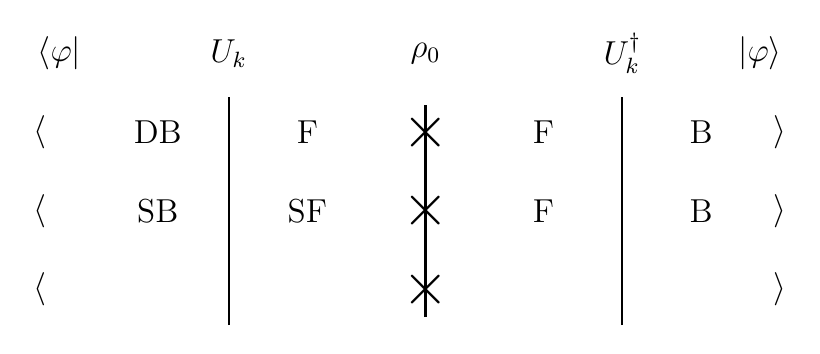
\begin{tikzpicture}[
    font=\large,
    every node/.style={inner sep=2pt},
]
% ---- column x-coordinates ----
\def\xbra{0}      % <phi|  and the three < bras
\def\xlab{1.5}    % DB / SB labels
\def\bL{2.4}      % left vertical bar of inner bracket
\def\xUk{3.4}     % U_k entries (F / SF)
\def\xrho{4.9}    % rho_0 spine with the three crosses
\def\xUkd{6.4}    % U_k^dagger entries (F / Fbar)
\def\bR{7.4}      % right vertical bar of inner bracket
\def\xB{8.4}      % |phi> entries (B / B)
\def\xket{9.4}    % the three > kets
 
% ---- row y-coordinates ----
\def\yh{3}        % header row
\def\yA{2}        % row 1
\def\yB{1}        % row 2
\def\yC{0}        % row 3
 
% ---- header labels ----
\node at (\xbra+0.25,\yh) {$\langle\varphi|$};
\node at (\bL  ,\yh) {$U_k$};
\node at (\xrho,\yh) {$\rho_0$};
\node at (\bR  ,\yh) {$U_k^{\dagger}$};
\node at (\xB+0.75,\yh) {$|\varphi\rangle$};
 
% ---- left bras ----
\node at (\xbra,\yA) {$\langle$};
\node at (\xbra,\yB) {$\langle$};
\node at (\xbra,\yC) {$\langle$};
 
% ---- DB / SB labels ----
\node at (\xlab,\yA) {DB};
\node at (\xlab,\yB) {SB};
 
% ---- left vertical bar ----
\draw[thick] (\bL,\yC-0.45) -- (\bL,\yA+0.45);
 
% ---- U_k column ----
\node at (\xUk,\yA) {F};
\node at (\xUk,\yB) {SF};
 
% ---- rho_0 spine with three crosses ----
\draw[thick] (\xrho,\yC-0.35) -- (\xrho,\yA+0.35);
\node[scale=1.8] at (\xrho,\yA) {$\times$};
\node[scale=1.8] at (\xrho,\yB) {$\times$};
\node[scale=1.8] at (\xrho,\yC) {$\times$};
 
% ---- U_k^dagger column ----
\node at (\xUkd,\yA) {F};
\node at (\xUkd,\yB) {F};   % second entry: change to {F} if it is just a plain F
 
% ---- right vertical bar ----
\draw[thick] (\bR,\yC-0.45) -- (\bR,\yA+0.45);
 
% ---- |phi> column ----
\node at (\xB,\yA) {B};
\node at (\xB,\yB) {B};
 
% ---- right kets ----
\node at (\xket,\yA) {$\rangle$};
\node at (\xket,\yB) {$\rangle$};
\node at (\xket,\yC) {$\rangle$};
 
    \end{tikzpicture}
\caption{The fluctuation summation can be decomposed as follows: the propagation chain is partitioned by $U_k$, $\rho_0$, and $U_k^\dagger$, which defines four possible insertion regions for each fluctuation operator. The two indistinguishable $V$ operators may be placed either in the same region or in different regions. In each region, the contribution can be double fluctuation ($DF$ or $DB$), single fluctuation ($SF$ or $SB$), or no fluctuation ($F$ or $B$). It is also worth to note that at second order, each chain contains exactly two fluctuation operators. }
\end{figure}
The diagram is for one fixed channel $a$, with its label suppressed. There are
11 second-order terms per channel; sum them over $a$ and add the closed term once.


\begin{align*}
    \closef = B^\dagger FF^\dagger B\\
    \mathcal{F} = \closef + \sum_a\Big[&DB_a^\dagger\, F\, F^\dagger\, B + h.c.\\
    + &SB_a^\dagger\, SF_a\, F^\dagger\, B + h.c.\\
    + &SB_a^\dagger\, F\, SF_a^\dagger\, B + h.c.\\
    + &SB_a^\dagger\, F\, F^\dagger\, SB_a \\
    + &B^\dagger\, DF_a\, F^\dagger\, B + h.c.\\
    + &B^\dagger\, SF_a\, SF_a^\dagger\, B\Big].
\end{align*}
At the final time, define $A_0=\braket{\psi}{F_N}$,
$A_{1,a}=\braket{\psi}{SF_{N,a}}$, and $A_{2,a}=\braket{\psi}{DF_{N,a}}$.
The same expression simplifies to
\begin{align}
\mathcal F &\approx |A_0|^2+\sum_a\left[|A_{1,a}|^2+
2\operatorname{Re}(A_0^* A_{2,a})\right],\\
\partial_c\mathcal F &=2\operatorname{Re}\left\{
A_0^*\partial_c A_0+\sum_a\left[
A_{1,a}^*\partial_c A_{1,a}+(\partial_c A_0)^*A_{2,a}
+A_0^*\partial_c A_{2,a}\right]\right\}.
\end{align}
Here $\partial_c$ denotes differentiation with respect to one control coordinate.
In particular, $\sum_a|A_{1,a}|^2$ must not be replaced by
$|\sum_a A_{1,a}|^2$. Weighted state-pair averaging is applied afterwards and
does not perform the noise average.
Introduce the notation
\begin{equation}
    \dvbar{F_k} = \pdv{\ket{F_k}}{\vb c(k)}
\end{equation}
Now differentiate the local recursions separately for each noise channel.

\begin{align*}
    \dvbar{F_k} &= \dvbar{W_k}\ket{F_{k-1}} \approx -i\tau H_c\ket{F_k},\\
    \dvbar{SF_{k,a}} &= \dvbar{W_k}\ket{SF_{k-1,a}} + \dvbar{V_{k,a}}\ket{F_{k-1}},\\
    \dvbar{DF_{k,a}} &= \dvbar{W_k}\ket{DF_{k-1,a}} + \dvbar{V_{k,a}}\ket{SF_{k-1,a}}.
\end{align*}

The derivatives of the propagators $W$ and $V$ can be calculated from the Fr\'echet derivative of the matrix exponential. With the condition $\kappa_1\ll 1$, we can use the Dyson expansion and keep only the first order term.
\begin{align}
    \pdv{W_k}{c_i(k)}
    &=
    -i\tau H_i W_k
    + O\!\left((\tau\norm{H})^2\right),
    \\
    \pdv{V_{k,a}}{c_i(k)}
    &= -i\tau\sigma_a\left[
    \pdv{H_a(t_k)}{c_i(k)}W_k+
    H_a(t_k)\pdv{W_k}{c_i(k)}\right].
\end{align}
The last identity differentiates the leading-insertion definition exactly.
For a static source the explicit derivative of $H_a$ is zero. For a relative
control source belonging to control $j$, it is $\delta_{ij}H_{\chi_j}$.
The derivative through $W_k$ contributes to every channel. Backward contraction
uses the same channel label on both sides before summing channel contributions.

\[\sigma_k=\sqrt{\sum_j \|H_{\mathrm{static},j}\|_2^2+\sum_a\left(
c_{k,a}\|H_{\mathrm{control\_fluc},a}\|_2
\right)^2}
\]


\[
\sigma_{\mathrm{rms}}
=
\sqrt{
\frac{1}{N}
\sum_k \sigma_k^2
}
\]
The leading-order fluctuation effect is $(\sigma_{\mathrm{rms}}T)^2$; defining $\kappa_2 = \sigma_{\mathrm{rms}}T$, we require $\kappa_2^2 \ll 1$ for the first-order approximation to be valid.


\subsection{Gradient with Decoherence}

For the short time correlation part, the noise is Markovian and is described
by the Lindblad superoperator
\begin{equation}
    \dot{\rho}(t)
    =
    -i[H(t),\rho(t)]
    +
    \mathcal{L}[\rho(t)] .
    \label{eq:lindblad_master_for_decoherence}
\end{equation}
Let $U(t,0)$ be the Hamiltonian propagator,
\begin{equation}
    i\dv{}{t}U(t,0) = H(t)U(t,0),
    \qquad
    U(0,0)=I.
\end{equation}
The closed-system trajectory is
\begin{equation}
    \rho_0(t)
    =
    U(t,0)\rho(0)U^\dagger(t,0).
\end{equation}
To isolate the decoherence contribution, move to the Hamiltonian interaction
picture:
\begin{equation}
    \rho(t)
    =
    U(t,0)\widetilde{\rho}(t)U^\dagger(t,0),
    \qquad
    \widetilde{\rho}(t)
    =
    U^\dagger(t,0)\rho(t)U(t,0).
\end{equation}
Then the Hamiltonian part is removed and the remaining evolution is
\begin{equation}
    \partial_t\widetilde{\rho}(t)
    =
    \widetilde{\mathcal{L}}(t)[\widetilde{\rho}(t)],
\end{equation}
where the interaction-picture Lindblad superoperator is
\begin{equation}
    \widetilde{\mathcal{L}}(t)[\widetilde{\rho}]
    =
    U^\dagger(t,0)
    \mathcal{L}\!\left[
        U(t,0)\widetilde{\rho}U^\dagger(t,0)
    \right]
    U(t,0).
\end{equation}

The integral equation is
\begin{equation}
    \widetilde{\rho}(T)
    =
    \widetilde{\rho}(0)
    +
    \int_0^T
    \widetilde{\mathcal{L}}(s_1)[\widetilde{\rho}(s_1)]\dd s_1 .
\end{equation}
Iterating this equation gives a Dyson expansion in the decoherence strength:
\begin{align}
    \widetilde{\rho}(T)
    =
    \widetilde{\rho}(0)
    &+
    \int_0^T
    \widetilde{\mathcal{L}}(s_1)[\widetilde{\rho}(0)]\dd s_1
    \notag\\
    &+
    \int_0^T\dd s_1
    \int_0^{s_1}\dd s_2\,
    \widetilde{\mathcal{L}}(s_1)
    \widetilde{\mathcal{L}}(s_2)
    [\widetilde{\rho}(0)]
    + \cdots .
    \label{eq:lindblad_dyson_expansion}
\end{align}
Keeping only the first order decoherence correction,
\begin{equation}
    \widetilde{\rho}(T)
    \approx
    \rho(0)
    +
    \int_0^T
    \widetilde{\mathcal{L}}(s)[\rho(0)]\dd s .
\end{equation}
Transforming back to the Schr\"odinger picture gives
\begin{equation}
    \rho(T)
    \approx
    \rho_0(T)
    +
    \int_0^T
    U(T,s)\,
    \mathcal{L}[\rho_0(s)]\,
    U^\dagger(T,s)\dd s,
    \label{eq:first_order_lindblad_schrodinger}
\end{equation}
where $U(T,s)=U(T,0)U^\dagger(s,0)$. This $U(T,s)$ factor is important:
decoherence happens at the intermediate time $s$, and the remaining control
pulse still propagates the correction to the final time.

For GRAPE, take $T=N\tau$ and
\begin{equation}
    W_k = \exp\{-i\tau H(t_k)\}.
\end{equation}
Then
\begin{align}
    U(t_k,0) &= W_k W_{k-1}\cdots W_1,\\
    U(T,t_k) &= W_N W_{N-1}\cdots W_{k+1}.
\end{align}
The first order correction becomes
\begin{equation}
    \rho(T)
    \approx
    \rho_0(T)
    +
    \tau
    \sum_{k=1}^{N}
    U(T,t_k)\,
    \mathcal{L}[\rho_0(t_k)]\,
    U^\dagger(T,t_k).
    \label{eq:discrete_lindblad_correction}
\end{equation}
For a pure initial state $\rho(0)=\ketbra{\psi_0}$, define
\begin{align}
    \ket{F_k}
    &=
    U(t_k,0)\ket{\psi_0}
    =
    W_k\cdots W_1\ket{\psi_0},
    \\
    \bra{B_k}
    &=
    \bra{\psi_T}U(T,t_k)
    =
    \bra{\psi_T}W_N\cdots W_{k+1}.
\end{align}
The target-state fidelity is
\begin{equation}
    \mathcal{F}
    =
    \mel{\psi_T}{\rho(T)}{\psi_T}.
\end{equation}
Therefore the first order decoherence correction is localized on each time
slice:
\begin{equation}
    \delta \mathcal{F}_{\mathrm{dec}}
    =
    \tau
    \sum_{k=1}^{N}
    \mel{B_k}{
        \mathcal{L}[\ket{F_k}\bra{F_k}]
    }{B_k}.
    \label{eq:decoherence_fidelity_correction}
\end{equation}
This is the clean GRAPE form: the density matrix does not need to be
propagated explicitly, because the correction can be contracted using the
forward state $\ket{F_k}$ and the backward state $\bra{B_k}$.

For one Lindblad jump operator $L$,
\begin{equation}
    \mathcal{L}[\rho]
    =
    L\rho L^\dagger
    -
    \frac{1}{2}L^\dagger L\rho
    -
    \frac{1}{2}\rho L^\dagger L .
\end{equation}
Substituting $\rho=\ket{F_k}\bra{F_k}$ into
Eq.~\eqref{eq:decoherence_fidelity_correction} gives
\begin{align}
    \delta \mathcal{F}_{\mathrm{dec}}
    &=
    \tau
    \sum_{k=1}^{N}
    \Big[
    \abs{\mel{B_k}{L}{F_k}}^2
        -
        \frac{1}{2}
        \mel{B_k}{L^\dagger L}{F_k}
        \braket{F_k}{B_k}
        -
        \frac{1}{2}
        \braket{B_k}{F_k}
        \mel{F_k}{L^\dagger L}{B_k}
    \Big].
    \label{eq:single_lindblad_decoherence_fidelity}\\
    \delta \mathcal{F}_{\mathrm{dec}} &= \tau \sum_{j=1}^{N} \mel**{\phi_T}{W_N\cdots J_j \cdots W_1}{\ket{\psi_0}}\mel{\psi_0}{W_1^\dagger \cdots J_j^\dagger \cdots W_N^\dagger}{\phi_T} \\
    &+\mel**{\phi_T}{W_N\cdots K_j\cdots W_1}{\psi_0}\mel{\psi_0}{U^\dagger(T)}{\phi_T}\notag\\
     &+\mel{\phi_T}{U(T)}{\psi_0}\mel**{\psi_0}{W_1^\dagger \cdots K_j^\dagger \cdots W_N^\dagger}{\phi_T}\notag\\
     \pdv{\delta \mathcal{F}_{\mathrm{dec}}}{c(k)} &= \tau \sum_{j=1}^{N}\mel**{\phi_T}{W_N\cdots J_j \dvbar{W_k} \cdots W_1}{\psi_0}\mel{\psi_0}{W_1^\dagger \cdots J_j^\dagger \cdots W_N^\dagger}{\phi_T} \\ 
     &+ \mel**{\phi_T}{W_N\cdots K_j \dvbar{W_k} \cdots W_1}{\psi_0}\mel{\psi_0}{U^\dagger(T)}{\phi_T}\notag\\
     &+\mel**{\phi_T}{W_N\cdots \dvbar{W_k} \cdots W_1}{\psi_0}\mel{\psi_0}{W_1^\dagger \cdots K_j^\dagger \cdots W_N^\dagger}{\phi_T} \notag\\
     &+\text{c.c.}
\end{align}
% REVIEW: dangling sentence "This has form of" -- incomplete.
where $J_j = L W_j$ and $K_j = -(1/2)L^\dagger L W_j$. This has form of

For multiple decoherence channels,
\begin{align}
    \delta \mathcal{F}_{\mathrm{dec}}
    &=
    \tau
    \sum_{k=1}^{N}
    \sum_{\mu}
    \Big[
        \abs{\mel{B_k}{L_\mu}{F_k}}^2
        -
        \frac{1}{2}
        \mel{B_k}{L_\mu^\dagger L_\mu}{F_k}
        \braket{F_k}{B_k}
        -
        \frac{1}{2}
        \braket{B_k}{F_k}
        \mel{F_k}{L_\mu^\dagger L_\mu}{B_k}
    \Big]
    \label{eq:multi_lindblad_decoherence_fidelity}\\
    % &= \tau \sum_{k=1}^{N}\sum_{\mu} \left[ \mel**{B_k}{\left(L_\mu\mel{F_k}{L_\mu^\dagger}{B_k} + (\mathbb{1} - \frac{1}{2}L_\mu^\dagger L_\mu)\mel{F_k}{(\mathbb{1} - \frac{1}{2}L_\mu^\dagger L_\mu)}{B_k}\right)}{F_k} \right]
    % REVIEW: conjugation error -- the last scalar in the braces (and in x_k below)
    % must be -\frac{1}{2}\mel{F_k}{L_\mu^\dagger L_\mu}{B_k}, i.e. the conjugate of
    % what is written, to reproduce eq. (multi_lindblad_decoherence_fidelity) above:
    % <B|x|F> then gives |a|^2 - Re(b s^*) with a = <B|L|F>, b = <B|L^dag L|F>,
    % s = <B|F>. As written it gives |a|^2 - b Re(s), which is complex in general.
    % The implementation (quantum_control/, doc/lindblad_note.md) uses the corrected form.
    &= \tau \sum_{k=1}^{N}\sum_{\mu}\mel**{B_k}{\left\{\mel{F_k}{L_\mu^\dagger}{B_k}L_\mu -\frac{1}{2}\braket{F_k}{B_k}L_\mu^\dagger L_\mu - \frac{1}{2}\mel{B_k}{L_\mu^\dagger L_\mu}{F_k}\right\}}{F_k}
    \intertext{denote $x_k = \mel{F_k}{L_\mu^\dagger}{B_k}L_\mu -\frac{1}{2}\braket{F_k}{B_k}L_\mu^\dagger L_\mu - \frac{1}{2}\mel{B_k}{L_\mu^\dagger L_\mu}{F_k}$, we have}
    \delta \mathcal{F}_{\mathrm{dec}}
    &=
    \tau \sum_{k=1}^{N}\sum_{\mu}\mel{B_k}{x_k}{F_k}
    \label{eq:multi_lindblad_decoherence_fidelity_2}
\end{align}
The closed-system fidelity can be written as
\begin{equation}
    \mathcal{F}_0
    =
    \abs{\braket{B_k}{F_k}}^2,
\end{equation}
which is independent of $k$ because the forward and backward pieces compose
to the full propagator. With decoherence,
\begin{equation}
    \mathcal{F}
    \approx
    \mathcal{F}_0
    +
    \delta \mathcal{F}_{\mathrm{dec}}
    + O(\tau^2\norm{\mathcal{L}}^2).
\end{equation}
The derivative is then be
% REVIEW: two issues in the derivative line. (a) The second term should be
% \braket{B_k^{(1)}}{\dvbar{F_k^{(0)}}} (the single-insertion backward state paired
% with the derivative of the plain forward chain), consistent with the lemma
% \dvbar{\mathcal{F}^{(l)}} = \sum_{m+n=l}\braket{B_k^{(m)}}{\dvbar{F_k^{(n)}}},
% not the derivative of B^{(1)}; the diagonal insertion contribution
% <B_k^{(0)}|x_k\dvbar{W_k}|F_{k-1}^{(0)}> from \dvbar{V_k} = x_k\dvbar{W_k} enters
% through \dvbar{F_k^{(1)}}. (b) This recursion is exact only with the
% frozen-coefficient reading: the scalars inside x_k depend on all controls, but
% freezing them and adding +c.c. reproduces the exact gradient term-by-term,
% provided the conjugation of x_k flagged above is corrected.
% See doc/lindblad_note.md, Sec. 6, for the verified statement.
\begin{align*}
    \pdv{\mathcal{F}}{c(k)} = \braket{B_k}{\dvbar{F_k^{(1)}}} + \braket{\dvbar{B_k^{(1)}}}{F_k} + \text{c.c.}
\end{align*}
where $F_k^{(1)} = x_k W_k\ket{F_{k-1}} + W_k\ket{F_{k-1}^{(1)}}$
\section{Experiment: Ion Trap and Laser Interaction}
Consider a system of $2$ ions in a linear trap (Paul trap). There exist two collective motional modes along each axis: the COM mode and the stretch mode. The COM mode is the one where the two ions move in phase, while the stretch mode is the one where they move out of phase. The frequencies of these modes are different. The COM mode has a frequency $\omega_{COM}$, while the stretch mode has a frequency $\omega_{stretch}$. 
If an outer magnetic field is applied, ions will have a Zeeman splitting. The qubit could be encoded in this Zeeman splitting level, directly by two fine structure levels. The first will use radio frequency (RF) to drive the transition between the two levels. The second will use Raman transition to drive the transition between the two levels.

The interaction:
\begin{equation}
    E_{int} = \vb d \cdot \vb E = \sum_{i,j} \bra{i} \vb x \ket{j} \ket{i}\bra{j} \cdot (-e\vb E) = \hslash\Omega\sigma_x 
\end{equation}
An external laser field can be applied to the ions. The interaction between an $x$-polarized, $z$-propagating laser and the ions can be described by the Hamiltonian (written in the Hilbert space of the internal states of the ions and the motional states of the ions):
\begin{equation}
H =  \omega_k a_k^\dagger a_k +  \frac{\omega_0}{2} \sigma_z +  {\Omega} \cos(k x - \omega t + \phi)\sigma_x \quad \text{(set $\hslash = 1$)}
\end{equation}


where $\Omega$ is the Rabi frequency for the laser interacting with the certain ion, $k$ is the wavevector of the laser, $x$ is the position of the ion, $\omega$ is the frequency of the laser, and $\phi$ is the phase of the laser. 
It is easy to be confused that when the laser is time-dependent, the external field should be changed. 
Here is the hamiltonian after extend to the time-dependent laser field:
\begin{equation}
H =  \omega_k a_k^\dagger a_k +  \frac{\omega_0}{2} \sigma_z +  {\Omega} \cos(k x - {\int_0^t\omega(s) \dd s} + \phi(t))\sigma_x 
\end{equation}

The position of the ion can be quantized as $x = x_0 (a_k + a_k^\dagger)$, where $x_0$ is the size of the motional state of the ion determined by the trap frequency, $a_k$ and $a_k^\dagger$ are the annihilation and creation operators of the motional mode $k$. Use the transformation $\cos\theta = \frac{1}{2} (e^{i\theta} + e^{-i\theta})$, we can rewrite the Hamiltonian as:
\begin{equation}
    H =  \omega_k a_k^\dagger a_k +  \frac{\omega_0}{2} \sigma_z +  \frac{\Omega}{2} (e^{i(k x - \omega t + \phi)} + e^{-i(k x - \omega t + \phi)})\sigma_x 
\end{equation}

Change into interaction picture w.r.t. $H_0 = \omega_k a_k^\dagger a_k +  (\flatfrac{\omega_0}{2}) \sigma_z$, $U = e^{-i H_0 t}$, we have the transformation of the Hamiltonian:
\begin{equation}
    H \to H_I = U^\dagger H U - i U^\dagger \dot{U}
\end{equation}
use the relation 
\begin{equation}
    e^{i\theta A} = \cos\theta + i \sin\theta A \quad \text{if $A^2 = 1$, i.e., $A = \vb* \sigma \cdot \hat{n}$}
\end{equation}
we can get the following operator transformation:
\begin{align}
    \ket{a}\bra{b} \to e^{i(\omega_a - \omega_b) t} \ket{a}\bra{b}\quad \text{for bosonic operators}
\end{align}
\begin{align*}
    \begin{split}
    a_k &\to  e^{-i \omega_k t} a_k \\
    a_k^\dagger &\to e^{i \omega_k t} a_k^\dagger \\
    \sigma_+ &\to e^{i \omega_0 t} \sigma_+ \\
    \sigma_- &\to e^{-i \omega_0 t} \sigma_-
    \end{split}
\end{align*}
The interaction Hamiltonian can be easily calculated as:
\begin{equation}
    H_I =  \frac{\Omega}{2} \left\{\exp i \left(k x_0 (a_k e^{-i \omega_k t} + a_k^\dagger e^{i \omega_k t}) - \omega t + \phi\right) + h.c.\right\} (\sigma_+ e^{i \omega_0 t} + h.c.)
\end{equation}
If the external electric field frequency $\omega$ is near $\omega_0$, we apply the rotating wave approximation (RWA), drop the fast oscillating terms, and obtain the following Hamiltonian:
\begin{equation}
    H_{\textit{RWA}} =  \frac{\Omega}{2}\sigma_+ \left[\exp i \left(k x_0 (a_k e^{-i \omega_k t} + a_k^\dagger e^{i \omega_k t})\right)\right]e^{-i\Delta t}e^{i\phi} + h.c.  \tag{Hamiltonian with RWA}
\end{equation}
where $\Delta = \omega - \omega_0$ is the detuning of the laser frequency from the qubit internal frequency.

If the wave vector of the external electric field along the $z$ direction is small compared to the size of the motional state of the ion, i.e. $\eta = k x_0 \ll 1$, then we are in the Lamb-Dicke regime, and we can expand the exponential to first order:
\begin{equation}
    H_{LD} =  \frac{\Omega}{2}\sigma_+e^{i\phi} \left[1 + i \eta a_k e^{-i \omega_k t} + i\eta a_k^\dagger e^{i \omega_k t}\right]e^{-i\Delta t} + h.c.
     \tag{Hamiltonian with Lamb-Dicke Approximation}
\end{equation}
A more careful analysis for the Lamb-Dicke regime is shown as follows. We can expand the exponential to the third order:
\begin{equation}
    \exp(i\eta (a + a^\dagger)) = 1 + i\eta (a + a^\dagger) - \frac{\eta^2}{2} (a + a^\dagger)^2  + \cdots 
\end{equation}
Representing this operator in the Fock basis, we see that the diagonal elements are $1 - \frac{\eta^2}{2} (2n + 1)$, the elements above the diagonal are $i\eta \sqrt{n+1}$, the elements below the diagonal are $i\eta \sqrt{n}$, the elements above the second diagonal are $-\frac{\eta^2}{2} \sqrt{(n+1)(n+2)}$, the elements below the second diagonal are $-\frac{\eta^2}{2} \sqrt{n(n-1)}$. Using the trace norm of the operator, one can conclude that a good approximation to second order requires $\eta\sqrt{\bar n + 1} \ll 1$, where $\bar n$ is the average phonon number of the motional state.

We can now define three kinds of external electric field: the carrier, the red sideband, and the blue sideband, which satisfy $\Delta = 0$, $\Delta = - \omega_k$, and $\Delta = \omega_k$, respectively. Each of them gives a different effective Hamiltonian after applying the RWA.
\begin{align}
    \begin{cases*}
    H_{carrier} = \frac{\Omega}{2} \sigma_+ e^{i\phi}e^{-i\Delta t} + h.c. \\
    H_{red} = i \frac{\Omega}{2} \eta \sigma_+ e^{i\phi} a_k e^{-i(\Delta + \omega_k) t} + h.c. \\
    H_{blue} = i \frac{\Omega}{2} \eta \sigma_+ e^{i\phi} a_k^\dagger e^{-i(\Delta - \omega_k) t} + h.c.
    \end{cases*}
\end{align}
Applying a bichromatic electric field with detunings $\Delta_{r} = - \omega_k - \delta$ and $\Delta_{b} = \omega_k + \delta$, we get the following Hamiltonian:
\begin{equation}
    H_{bi} = (i \frac{\Omega}{2} \eta \sigma_+ e^{i\phi_r} a_k e^{i\delta t} + h.c.) + (i \frac{\Omega}{2} \eta \sigma_+ e^{i\phi_b} a_k^\dagger e^{-i\delta t} + h.c.)
\end{equation}
Define $\phi_s = \frac{\phi_r + \phi_b + \pi}{2}$, $\phi_m = \frac{\phi_b - \phi_r}{2}$, we can rewrite the Hamiltonian as:
\begin{equation}
    H_{bi} = ( \frac{\Omega}{2} \eta \sigma_+ e^{i(\phi_s - \phi_m)} a_k e^{i\delta t} + h.c.) + ( \frac{\Omega}{2} \eta \sigma_+ e^{i(\phi_s + \phi_m)} a_k^\dagger e^{-i\delta t} + h.c.)
\end{equation}
We finally get the effective Hamiltonian of one ion interacting with a bichromatic laser coupling to mode $k$:
\begin{align}
    H_k &= \frac{\Omega}{2} \eta (\sigma_+ e^{i\phi_s} + \sigma_- e^{-i\phi_s})(a_k e^{i(\delta t - \phi_m)} + a_k^\dagger e^{-i(\delta t - \phi_m)})
\end{align}
\begin{notebox}
There exists global phase of bichromatic laser because this ``global'' is just global through the spin space. Since the system is considering the interaction between the motion and spin, this ``global'' phase is actually the phase difference between motion phase and laser phase. At the time reference $t=0$. Notice, this global phase can be removed if we define the real spin direction as $\sigma_x$. So this is just a redundance of the notation.  
\end{notebox}
Define following two operators:
\begin{equation}
    \begin{cases}
        \sigma_{\phi_s} = \sigma_+ e^{i\phi_s} + \sigma_- e^{-i\phi_s} \\
        A_{k, \phi_m}(t) = a_k e^{i(\delta t - \phi_m)} + a_k^\dagger e^{-i(\delta t - \phi_m)}
    \end{cases}\qquad \qquad 
    \begin{cases}
        \sigma_{\phi_s} = \sigma_+ e^{i\phi_s} + \sigma_- e^{-i\phi_s} \\
        A_{k, \phi_m}(t) = a_k e^{i\Phi_k(t)} + a_k^\dagger e^{-i\Phi_k(t)}
    \end{cases}
\end{equation}
Under the assumption that two laser have exactly the same detuning magnitude, $\phi_s$ will always be locked at the same value, thus the spin direction is fixed.  
we can rewrite the Hamiltonian as:
\begin{equation}
        H_k = \frac{\Omega}{2} \eta \cdot\sigma_{\phi_s}\otimes A_{k, \phi_m}(t) \tag{Effective Hamiltonian for bichromatic laser coupling}
\end{equation}


The sum of the phases determines the spin direction, while the difference of the phases determines the direction of the motional trajectory in phase space.

When the collective motional mode is considered for two ions, and the external electric field is applied to both ions, the effective Hamiltonian can be written as:
\begin{equation}
    H = \frac{\Omega}{2} \eta S_{\phi_s} \otimes A_{k, \phi_m}(t) \tag{Effective Hamiltonian for bichromatic laser coupling with two ions}
\end{equation}
where $S_\phi = \vb b_k \cdot \vb*\sigma_\phi$ and $\vb b_k$ is the mode vector of mode $k$. For the COM mode, $\vb b_k = (1,1)/2$; for the stretch mode, $\vb b_k = (1,-1)/2$. Notation: $S^+$ denotes the COM mode, $S^-$ denotes the stretch mode.
% REVIEW: the mode vectors $(1,\pm1)/2$ are not unit-normalized ($\lVert\vb b_k\rVert = 1/\sqrt2$). Confirm this is the intended normalization rather than $(1,\pm1)/\sqrt2$.

For the stretch mode, the two ions will move in opposite direction, so the effective Hamiltonian can be written as:
\begin{equation}
    H_{\textit{stretch}} = \frac{\Omega}{2} \eta \cdot \frac{1}{2}(\sigma_{\phi_s}^{(1)} - \sigma_{\phi_s}^{(2)}) \otimes (a_k e^{i(\delta t - \phi_m)} + a_k^\dagger e^{-i(\delta t - \phi_m)})
\end{equation}

\begin{notebox}[title=Rotating Frame Transformation]
    Consider the system $H(t) = H_0(t) + W(t)$, we want to apply the rotating frame transformation with $H_0(t)$, i.e., $U = \mathcal{T} e^{-i \int_0^t H_0(\tau) d\tau}$, where $\mathcal{T}$ is the time-ordering operator. The transformed Hamiltonian can be calculated as:

Note that for any unitary familty $V(t)$ ($VV^\dagger = V^\dagger V = \vb 1$,  $V(0) = \vb 1$ and is strong differentiable, i.e., $\dot V$ is well defined w.r.t. strong convergence), we can define a unitary transformation:
\begin{align*}
    \ket{\tilde\psi(t)} &= V^\dagger(t)\ket{\psi(t)}\\
    \tilde H &= V^\dagger H V - i V^\dagger \dot V 
\end{align*}
And the SE is preserving:
\begin{align*}
    i\partial_t \ket{\tilde\psi(t)} = \tilde H \ket{\tilde\psi(t)}
\end{align*}
If the unitary family $V$ is the propagator of a time-dependent Hamiltonian $H_0(t) = f(t)H_0$, it is commuting with itself at different time, i.e., $[H_0(t), H_0(t')] = 0$, then we can drop the time-ordering operator, and get the following transformation:
\begin{equation}
    V = \mathcal{T}\exp(-i \int_{t_0}^{t}H_0(\tau)\dd \tau) = \exp(-i(\int_{t_0}^{t}f(\tau)\dd \tau)H_0)
\end{equation}
Then the transformed Hamiltonian can be calculated as:
\begin{align*}
    \tilde H(t) &= V^\dagger H V - i V^\dagger \dot V \\
    &= V^\dagger H V - i V^\dagger (-ifH_0)V\\
    &= V_t^\dagger (H(t) - f(t)H_0) V_t
\end{align*}
\end{notebox}

Let $H_0(t) = (\delta + \delta't + \phi'_m)  a_k^\dagger a_k$, we can get the following transformation:
\begin{align*}
    H_{\text{stretch}} & \to \tilde H_{\text{stretch}} = - (\delta + \delta't + \phi'_m)a_k^\dagger a_k + \frac{\Omega}{2} \eta S_{\phi_s} \otimes (a_k + a_k^\dagger)
\end{align*}
We can use two simple parameter to represent the Hamiltonian $\alpha_1(t),\alpha_2(t)$:
\begin{align*}
    H = \alpha_1 \hat n_k + \alpha_2 S_{\phi_s} \otimes \hat x_k
\end{align*}
but the boundary condition of the control parameters should be carefully considered. A complex transformation from the experimental limit to the boundary condition of the control parameters is needed.

\subsection{Configuration}
The system evolves under the following Hamiltonian:
\begin{equation}
    H = \alpha_1(t) (1 + \chi_1)\hat n + \alpha_2(t) \eta(1+\chi_2)S^-_{\phi_s} \otimes \hat x_k + \xi_1 S_{\phi_s}^{+} + \xi_2 \hat n 
\end{equation}

The bounds on the control parameters and the standard deviations of the fluctuations are given as follows:
% REVIEW: the experiment configs (experiments/spin_boson/configs/*.yaml) use alpha_1 in 2pi*[1, 60] kHz and alpha_2 in 2pi*[0, 200] kHz — the 600/20 below look like transposed zeros.
% REVIEW: the configured value of sigma(xi_2) is 30 rad/s (approx 2pi * 4.8 Hz), not 2pi * 20 Hz.
\begin{align*}
    &\alpha_1\in 2\pi \cdot[1, 60] kHz \\
    &\alpha_2\in 2\pi \cdot[0, 200] kHz \\
    &\alpha_2(0) = \alpha_2(T) = 0 \\
    &\sigma(\chi_1) = 0.0001,\quad \sigma(\chi_2) = 0.0001 \\
    &\sigma(\xi_1) = 2\pi \cdot 5Hz,\quad \sigma(\xi_2) = 2\pi \cdot 20Hz\\
    & T = 225.8 \mu s
\end{align*}
\subsection{Experiment 1: pulse searching}
\paragraph{Historical results.}
The numerical tables and plots below were generated before the independent-channel
averaging correction of 2026-09-14. They are retained as historical results of
the earlier aggregate-insertion objective, not recomputed results of the corrected
derivation above. Claims about independent-noise robustness require reevaluation
with the corrected engine and the original pulse/configuration snapshots.

GRAPE is a local gradient method: from a given initial guess, L-BFGS-B converges to a stationary point inside the basin of attraction of that guess, so a single run samples exactly one basin of the control landscape. Experiment 1 therefore searches over basins. We prepared a gallery of ten named initial pulses --- sinusoidal $\alpha_2$ envelopes of different periods (\texttt{sine\_60}, \texttt{sine\_100}, \texttt{sine\_160}), multi-lobe envelopes (\texttt{two\_lobe}, \texttt{multilobe\_3}, \texttt{gaussian\_lobe}), a chirped ramp (\texttt{chirp\_ramp}), a constant high-$\alpha_1$ profile (\texttt{high\_alpha1\_const}), a flat-top profile (\texttt{flattop}) and a smoothed random profile (\texttt{random\_smooth}) --- and optimized each one independently under an identical configuration, one task per initial pulse (Slurm job array on USTC-SCC). Figure~\ref{fig:exp1-gallery} shows the gallery and the resulting optimized pulses.

All runs share $T = 225.8\,\mu s$, $N = 400$ steps, and at most $400$ L-BFGS-B iterations with smoothness penalties $\lambda_{L1} = 5\times 10^{-4}$, $\lambda_{L2} = 10^{-4}$. The gate fidelity is averaged over $96$ weighted state pairs: the $16$ logical two-qubit states $\{\ket 0, \ket 1, \ket +, \ket{+i}\}^{\otimes 2}$, with each target resolved over the $6$ motional levels. This experiment used a \emph{strong}-fluctuation scenario, ten times the static deviations of the Configuration above: $\sigma(\xi_1) = 2\pi\cdot 50\,\mathrm{Hz} = 314.16\,\mathrm{rad/s}$, $\sigma(\xi_2) = 300\,\mathrm{rad/s}$, $\sigma(\chi_1)=\sigma(\chi_2)=10^{-4}$.

\begin{table}[htbp]
    \centering
    \begin{tabular}{lccc}
        \hline
        initial pulse & initial $\openf$ & final $\openf$ & final $\closef$ \\
        \hline
        \texttt{gaussian\_lobe}     & 0.685066 & 0.999022 & 0.999974 \\
        \texttt{sine\_60}           & 0.643901 & 0.998939 & 0.999999 \\
        \texttt{sine\_100}          & 0.683796 & 0.998861 & 0.999997 \\
        \texttt{random\_smooth}     & 0.674495 & 0.998807 & 0.999982 \\
        \texttt{two\_lobe}          & 0.714529 & 0.998803 & 1.000000 \\
        \texttt{sine\_160}          & 0.782220 & 0.998799 & 0.999998 \\
        \texttt{high\_alpha1\_const}& 0.584793 & 0.998746 & 0.999997 \\
        \texttt{multilobe\_3}       & 0.624254 & 0.998708 & 0.999992 \\
        \texttt{chirp\_ramp}        & 0.760213 & 0.998693 & 0.999998 \\
        \texttt{flattop}            & 0.949247 & 0.998656 & 0.999984 \\
        \hline
    \end{tabular}
    \caption{Pulse search over ten initial-pulse basins (strong fluctuations, $T = 225.8\,\mu s$), sorted by final noisy gate fidelity $\openf$. $\closef$ is the closed-system gate fidelity of the same optimized pulse.}
    \label{tab:exp1-search}
\end{table}

Table~\ref{tab:exp1-search} summarizes the search. The initial noisy fidelities span $0.58$--$0.95$, yet every basin converges to nearly the same place: final $\openf$ between $0.998656$ and $0.999022$ (a spread of only $4\times10^{-4}$), with closed fidelities $\closef \geq 0.99997$ throughout. Two conclusions follow. First, at fixed gate time the reachable noisy fidelity is essentially basin-independent: the residual infidelity of $\sim 10^{-3}$ is set by the strong quasi-static noise, not by the pulse shape. Second, the ranking at fixed $T$ does not predict which shape survives gate-time compression --- \texttt{flattop}, last in this table, becomes the clear winner of Experiment 2.

\begin{figure}[htbp]
    \centering
    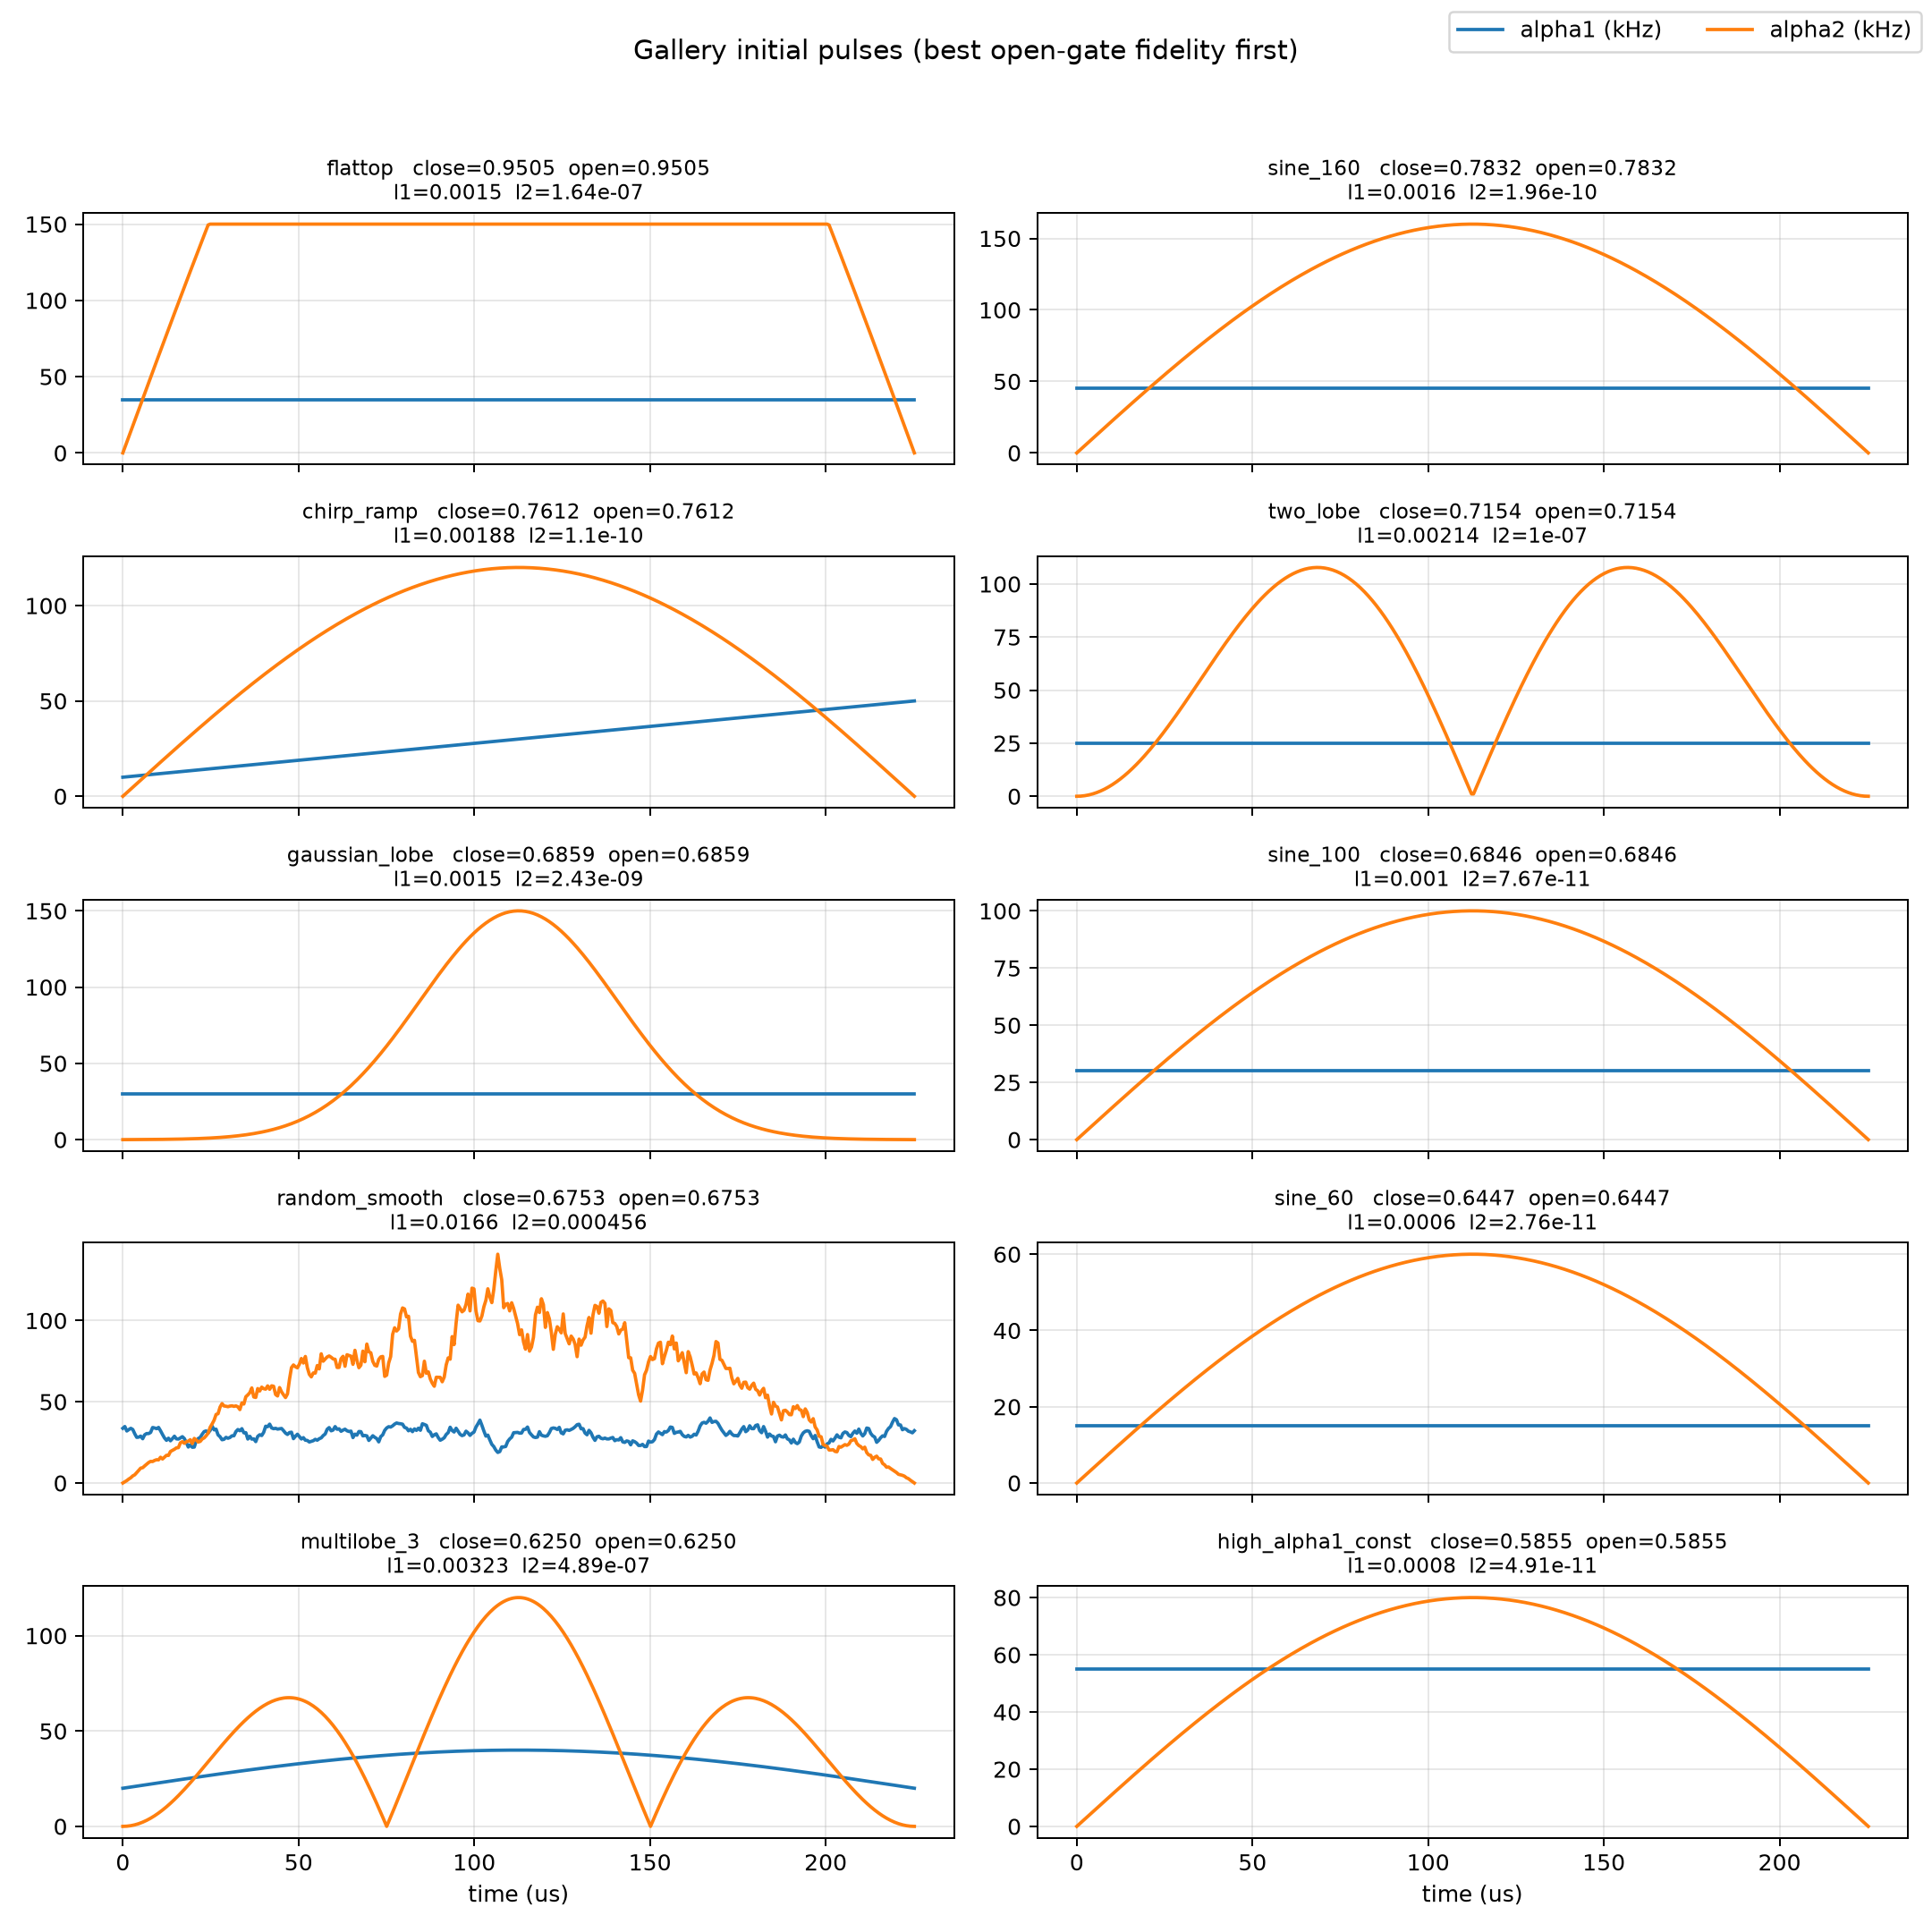
\includegraphics[width=0.78\textwidth]{../experiments/spin_boson/reports/src/preview.png}\\[4pt]
    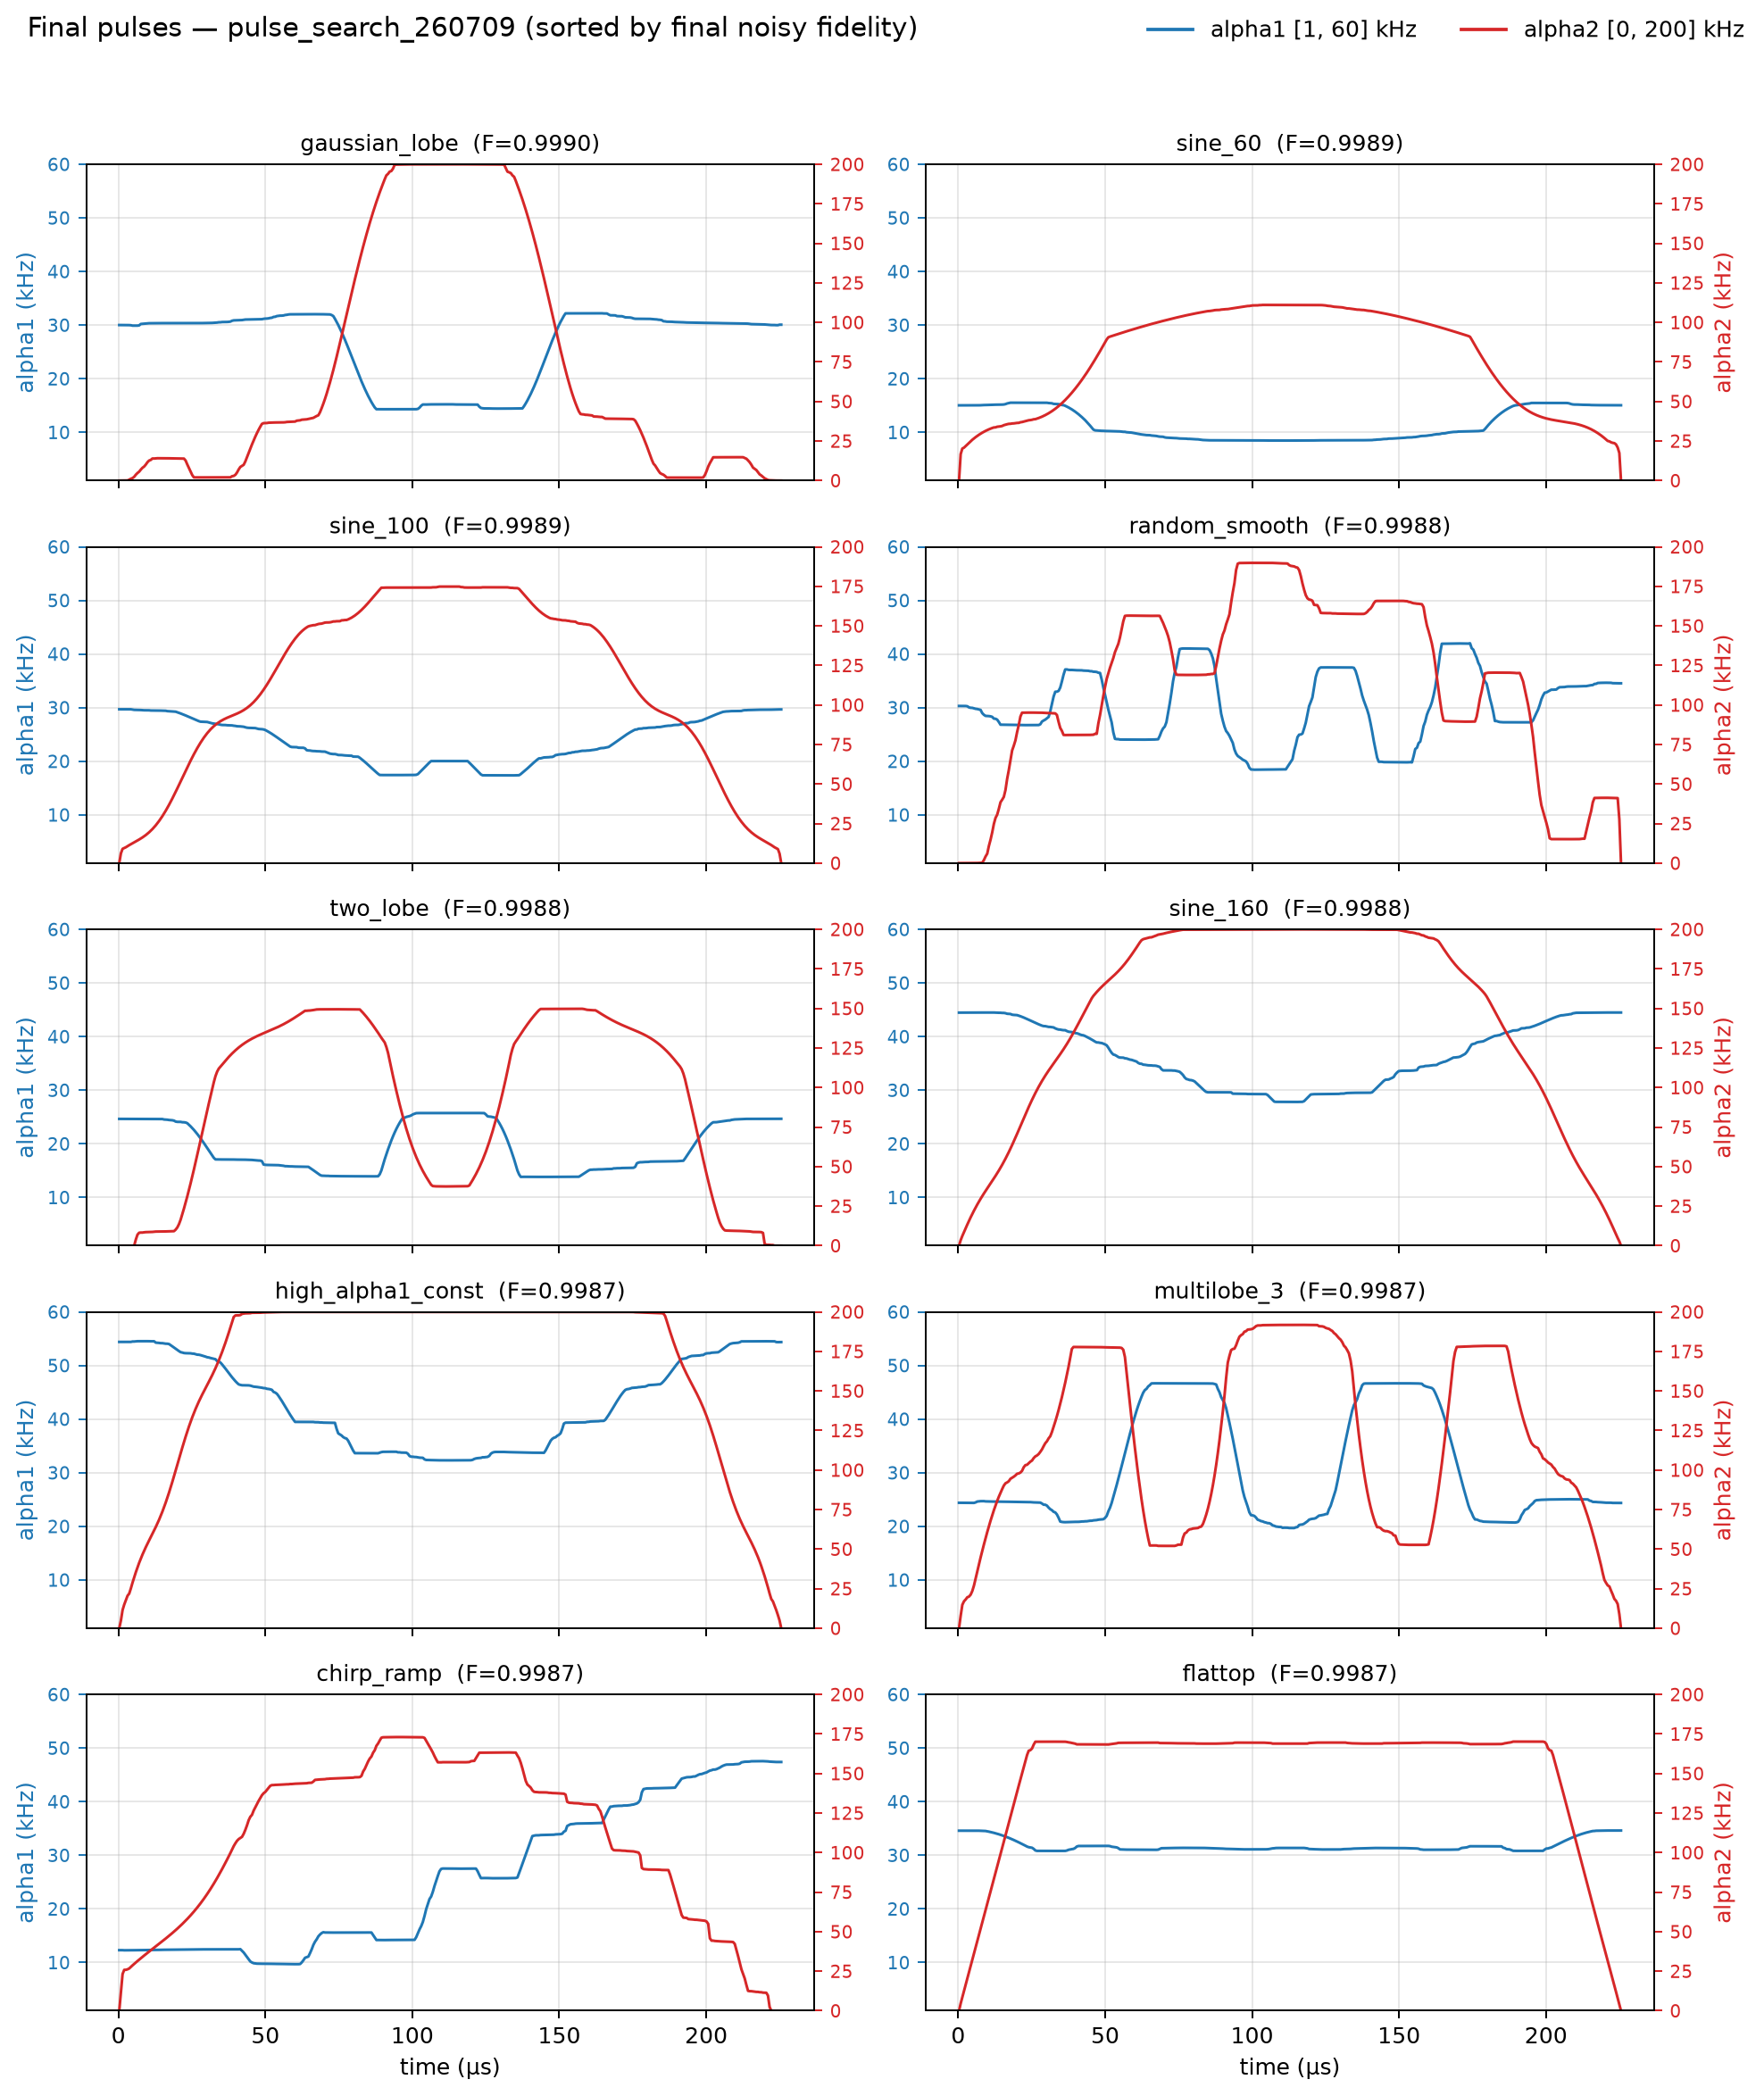
\includegraphics[width=0.7\textwidth]{../experiments/spin_boson/reports/src/final_pulses_grid.png}
    \caption{Experiment 1. Top: the gallery of initial pulses ($\alpha_1$, $\alpha_2$ per panel). Bottom: the corresponding optimized pulses; distinct basins yield visibly different waveforms at nearly identical fidelity.}
    \label{fig:exp1-gallery}
\end{figure}

\subsection{Experiment 2: time shrinking}
At leading order a quasi-static fluctuation contributes an infidelity $\propto (\sigma T)^2$, so a shorter gate is quadratically less sensitive --- provided re-optimization can keep the closed-system fidelity. Experiment 2 compresses the gate time by a multiplicative shrink loop: starting from an optimized pulse, each round sets $T \to 0.95\,T$ with $N = 400$ fixed (only the step duration shrinks; the amplitudes carry over), then re-optimizes warm-started from the previous round (at most $250$ iterations). The loop stops when the noisy gate fidelity drops more than $10^{-4}$ below the previous round, or after $30$ rounds; the reported result is the round with the highest $\openf$.

Every final pulse of Experiment 1 was fed through this loop from three starting gate times ($225.8$, $300$ and $170\,\mu s$), giving $30$ independent tasks (Slurm array). Unlike the search, this experiment used the \emph{weak}-fluctuation scenario of the Configuration: $\sigma(\xi_1) = 2\pi\cdot 5\,\mathrm{Hz} = 31.416\,\mathrm{rad/s}$, $\sigma(\xi_2) = 30\,\mathrm{rad/s}$. The jump in fidelity between Table~\ref{tab:exp1-search} and Table~\ref{tab:exp2-shrink} ($\openf \sim 0.999$ to $\openf > 0.9999$) reflects this change of noise level, not an improvement of the pulses.

\begin{table}[htbp]
    \centering
    \begin{tabular}{lcccc}
        \hline
        pulse & start $T$ ($\mu s$) & best $T$ ($\mu s$) & $\openf$ & $\closef$ \\
        \hline
        \texttt{flattop}            & 225.8 & \textbf{76.90} & 0.999998 & 0.999999 \\
        \texttt{gaussian\_lobe}     & 170   & 124.97 & 0.999941 & 0.999945 \\
        \texttt{high\_alpha1\_const}& 170   & 138.47 & 0.999995 & 0.999999 \\
        \texttt{sine\_160}          & 300   & 138.99 & 0.999996 & 1.000000 \\
        \texttt{sine\_100}          & 300   & 154.00 & 0.999995 & 1.000000 \\
        \texttt{random\_smooth}     & 170   & 161.50 & 0.999993 & 0.999999 \\
        \texttt{chirp\_ramp}        & 170   & 170.00 & 0.999978 & 0.999986 \\
        \texttt{multilobe\_3}       & 170   & 170.00 & 0.999992 & 0.999998 \\
        \texttt{sine\_60}           & 170   & 170.00 & 0.999947 & 0.999954 \\
        \texttt{two\_lobe}          & 170   & 170.00 & 0.999988 & 0.999996 \\
        \hline
    \end{tabular}
    \caption{Time shrinking (weak fluctuations): for each pulse, the shortest best gate time reached over the three starting times, with the fidelities of that round. Rows with best $T = 170\,\mu s$ started there and never improved on the starting time; fidelity values are as logged (rounded to six digits).}
    \label{tab:exp2-shrink}
\end{table}

Table~\ref{tab:exp2-shrink} lists, for each pulse, the shortest gate time reached over the three starts. Most shapes stall between $125$ and $170\,\mu s$. The \texttt{flattop} pulse is the outlier: starting from $225.8\,\mu s$ it shrinks for $21$ consecutive rounds down to
\begin{equation*}
    T = 76.90\,\mu s, \qquad \openf = 0.999998, \qquad \closef = 0.9999994,
\end{equation*}
a $2.9\times$ compression of the original gate time, with perturbative validity parameters $\kappa_1 = 0.368$ and $\kappa_2 = 0.0285$ at the final duration. The stop criterion triggered at round $23$ ($\openf = 0.99936 < 0.99998 - 10^{-4}$), indicating that below ${\sim}77\,\mu s$ re-optimization within the amplitude bounds can no longer support the gate. Notably, the noisy fidelity \emph{increases} monotonically while shrinking (e.g.\ from $0.999962$ at $225.8\,\mu s$), as expected from the $(\sigma T)^2$ scaling of the dominant static fluctuations. Figure~\ref{fig:exp2-best} shows the fidelity--time trade-off across all $30$ tasks and the winning waveform.

\begin{figure}[htbp]
    \centering
    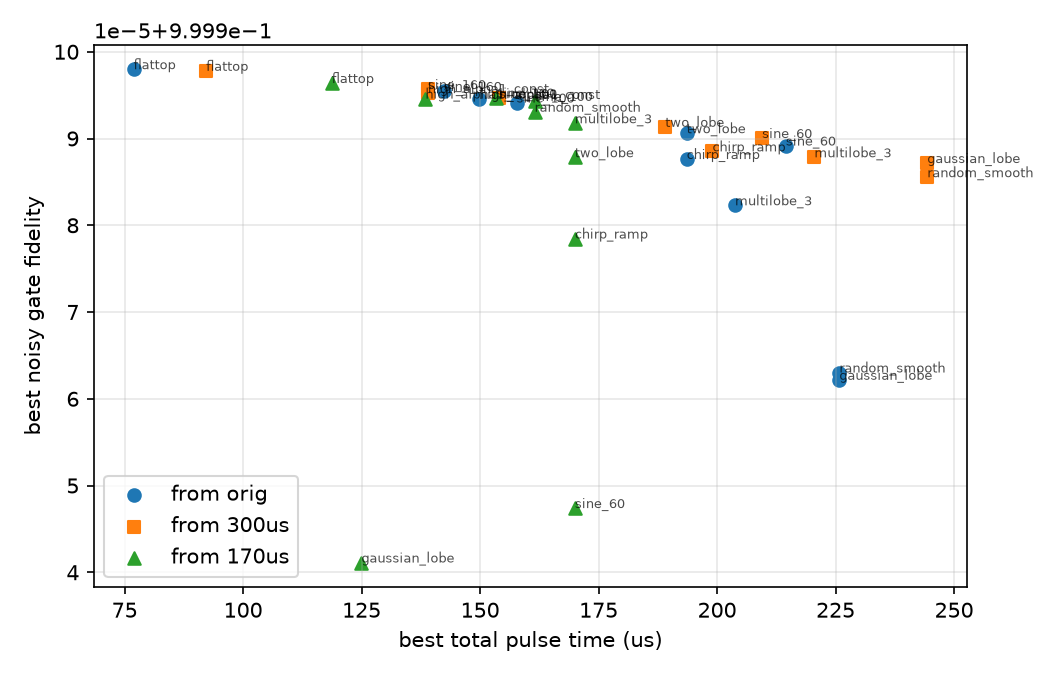
\includegraphics[width=0.62\textwidth]{../experiments/spin_boson/reports/src/best_time_vs_fidelity.png}\\[4pt]
    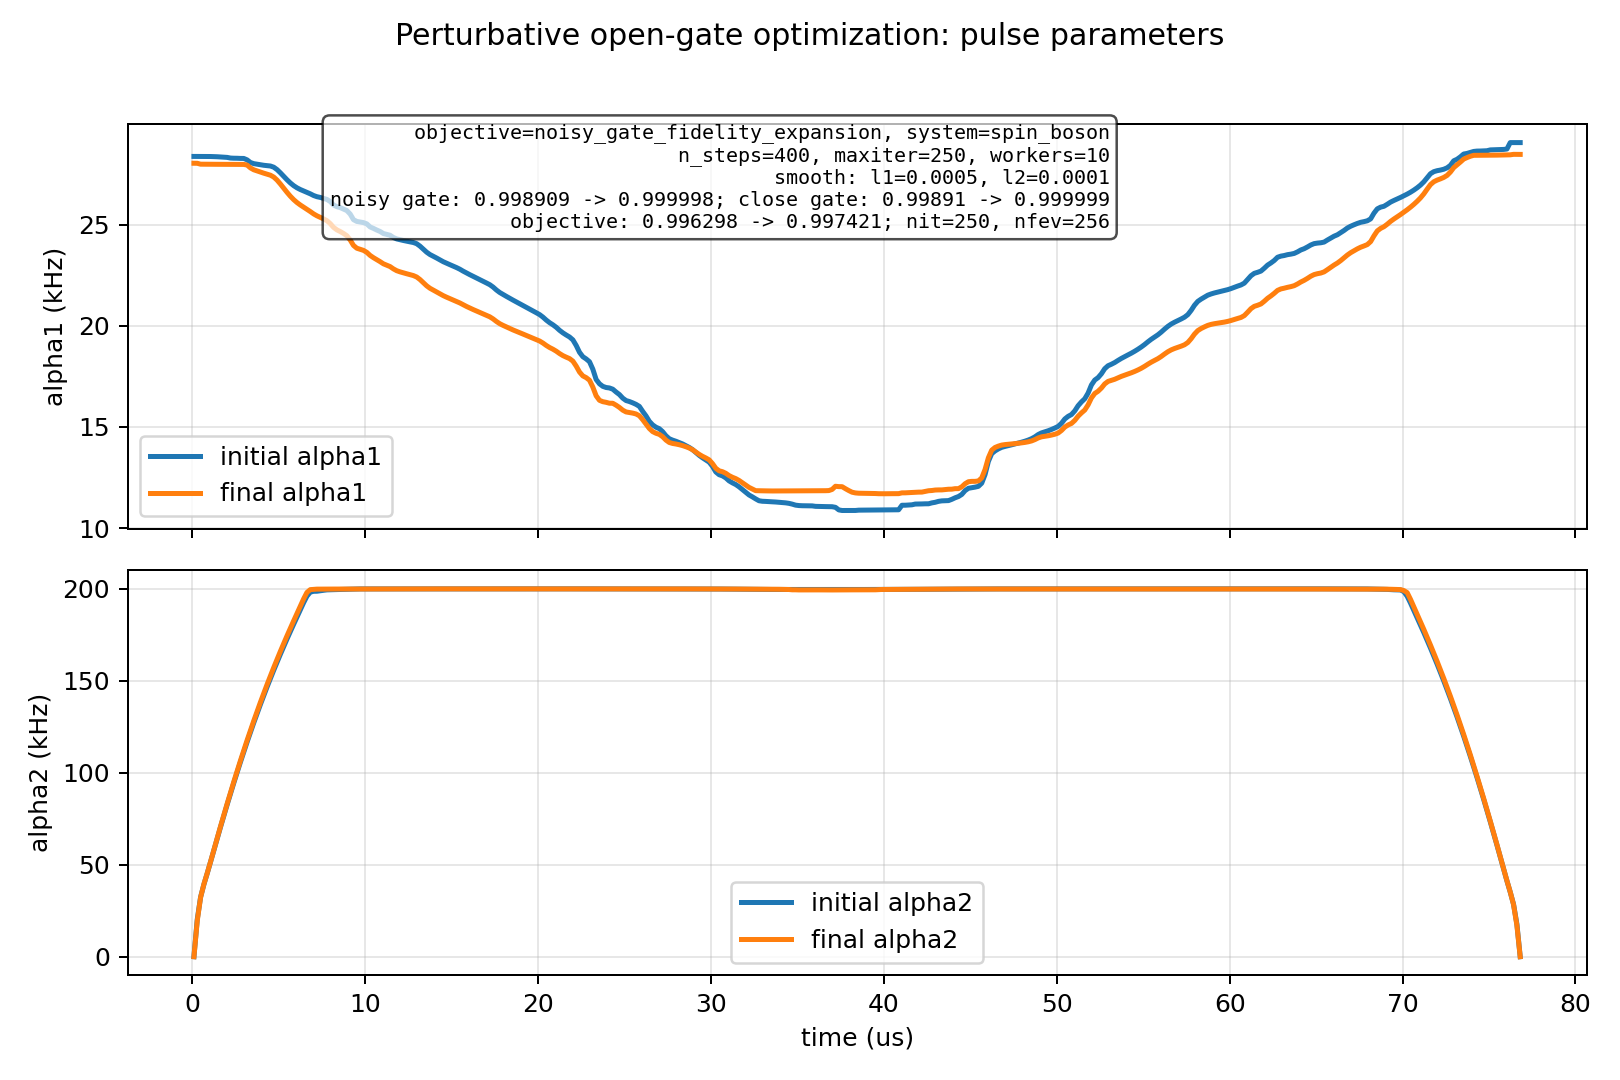
\includegraphics[width=0.49\textwidth]{../experiments/spin_boson/reports/src/round_21_T76.90us/pulse.png}\hfill
    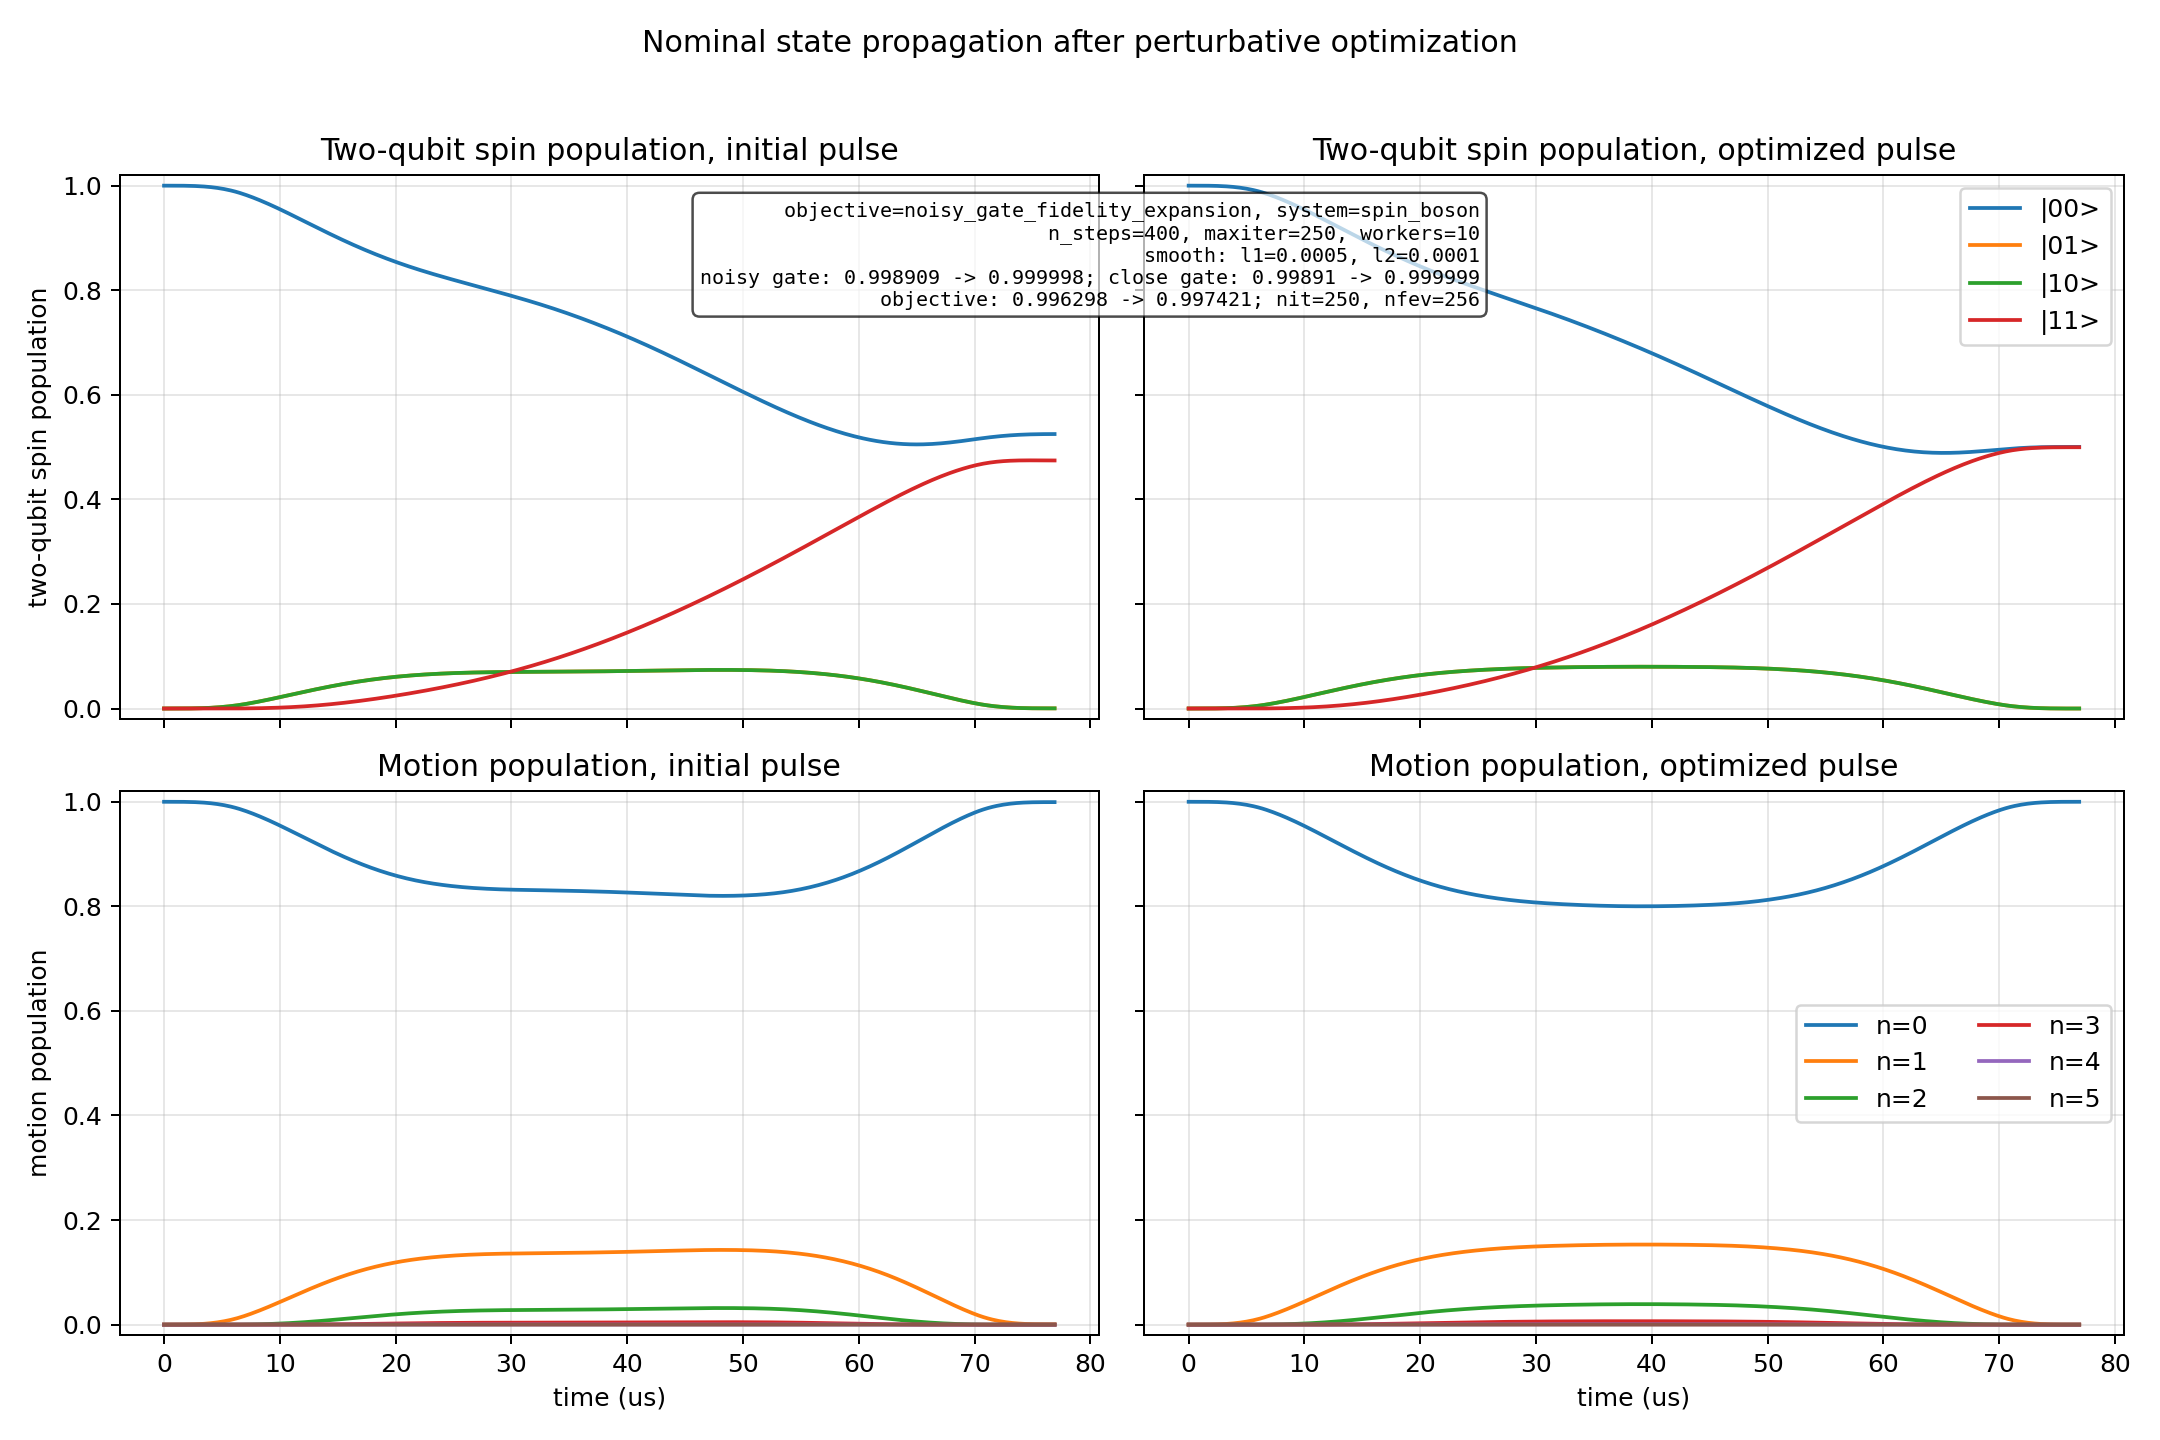
\includegraphics[width=0.49\textwidth]{../experiments/spin_boson/reports/src/round_21_T76.90us/population.png}
    \caption{Experiment 2. Top: best gate time vs.\ noisy fidelity for all $30$ shrink tasks. Bottom: the winning \texttt{flattop} pulse at $T=76.90\,\mu s$ (left) and the population evolution of the probe state $\ket{00}\otimes\ket{n=0}$ under it (right).}
    \label{fig:exp2-best}
\end{figure}

\subsection{Experiment 3: robustness evaluation}
Experiment 3 measures how the optimal pulse degrades as the noise grows. A global scale factor $\lambda$ multiplies all four fluctuation deviations simultaneously (decoherence stays disabled), and the pulse is evaluated at $30$ logarithmically spaced points $\lambda \in [0.01, 20]$ around the nominal weak-fluctuation scenario ($\lambda = 1$); the closed fidelity $\closef$ is the $\lambda \to 0$ asymptote. The evaluation is the same second-order perturbative $\openf$ used as the optimization objective, so large-$\lambda$ values are qualitative --- the expansion parameter itself grows as $(\lambda\sigma T)^2$.

The $76.90\,\mu s$ open-GRAPE pulse is compared against two closed-GRAPE references, i.e.\ pulses optimized with all noise terms disabled: one at the original $T = 225.8\,\mu s$, and one at the \emph{same} gate time $T = 76.90\,\mu s$. Each comparison pulse is evaluated on its own time grid under the identical scaled noise model.

\begin{table}[htbp]
    \centering
    \begin{tabular}{lcccc}
        \hline
        pulse & $T$ ($\mu s$) & $\closef$ & $\openf$ at $\lambda \approx 1.12$ & $\openf$ at $\lambda = 20$ \\
        \hline
        open-GRAPE (best)   & 76.90 & 0.99999941 & 0.99999762 & 0.999429 \\
        closed-GRAPE        & 76.90 & 0.99999951 & 0.99999769 & 0.999417 \\
        closed-GRAPE        & 225.8 & 0.99999937 & 0.99997989 & 0.993777 \\
        \hline
    \end{tabular}
    \caption{Robustness of the best pulse vs.\ two closed-GRAPE references under globally scaled fluctuations ($\lambda = 1$ is the nominal weak scenario).}
    \label{tab:exp3-robustness}
\end{table}

Table~\ref{tab:exp3-robustness} and Figure~\ref{fig:exp3-robustness} summarize the sweep. Three observations:
\begin{enumerate}
    \item The infidelity of the best pulse grows quadratically in $\lambda$, as expected for zero-mean quasi-static noise at second order; at the nominal $\lambda = 1$ the noise adds only ${\sim}2\times10^{-6}$ to the closed-system infidelity, and the fidelity stays above $0.9994$ even at $\lambda = 20$.
    \item Gate time dominates robustness. Against the $225.8\,\mu s$ reference the short pulse is ${\sim}11\times$ more robust at $\lambda = 20$ ($5.7\times10^{-4}$ vs.\ $6.2\times10^{-3}$ infidelity), consistent with the $(\sigma T)^2$ scaling of the static terms, $(225.8/76.9)^2 \approx 8.6$.
    \item At \emph{equal} gate time the open-GRAPE and closed-GRAPE pulses are equally robust to within a few percent at every $\lambda$. At this noise level, pulse shaping does not additionally suppress the static dephasing; the practical value of the open-system objective in this study is therefore not reshaping the pulse at fixed $T$, but steering and certifying the time-shrinking loop of Experiment 2, whose stop criterion is the noisy fidelity itself.
\end{enumerate}

\begin{figure}[htbp]
    \centering
    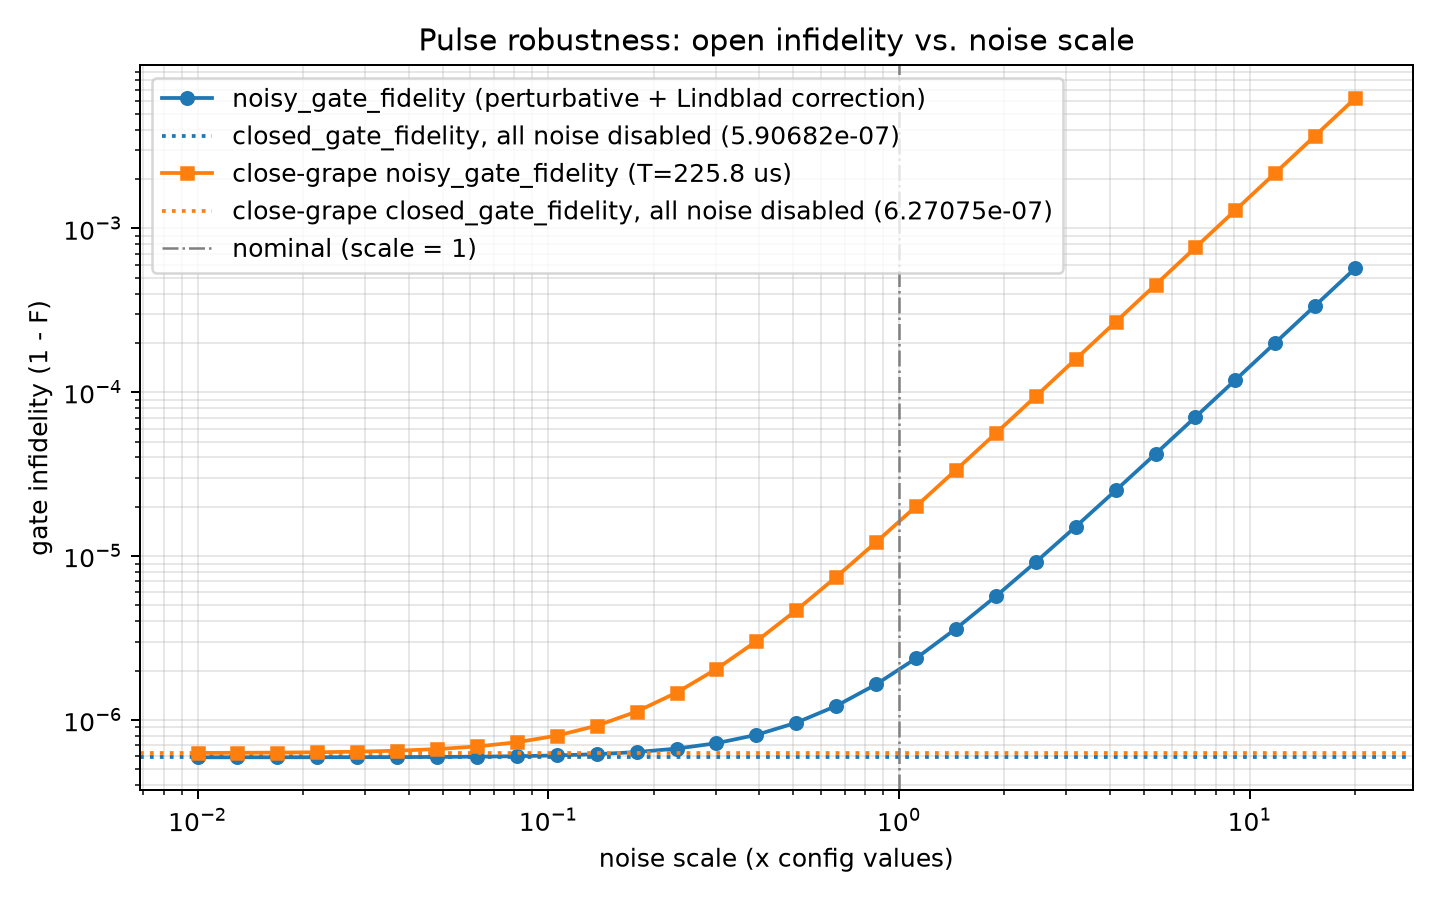
\includegraphics[width=0.75\textwidth]{../experiments/spin_boson/reports/src/robustness.png}\\[4pt]
    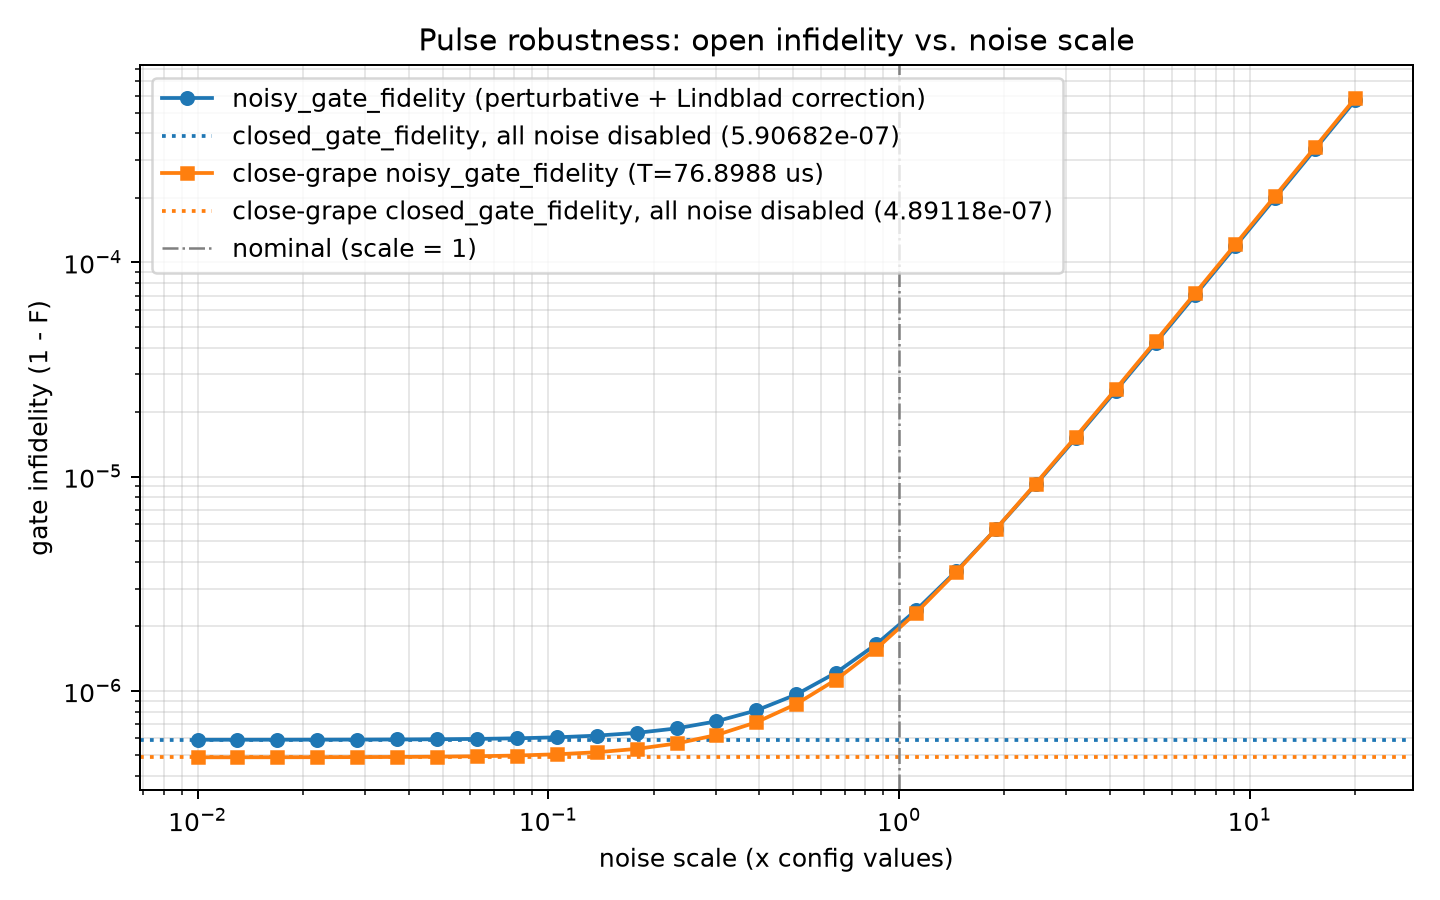
\includegraphics[width=0.75\textwidth]{../experiments/spin_boson/reports/src/robustness_same_time.png}
    \caption{Experiment 3: gate infidelity $1-\openf$ (log axis) vs.\ noise scale $\lambda$. Top: best $76.90\,\mu s$ pulse against the closed-GRAPE pulse at $225.8\,\mu s$. Bottom: the same against the closed-GRAPE pulse at the same $76.90\,\mu s$ gate time --- the two curves nearly coincide. Dotted lines mark the closed-fidelity ($\lambda \to 0$) references.}
    \label{fig:exp3-robustness}
\end{figure}

\subsection{Experiment 4: error budget analysis}



\nocite{*}
\printbibliography
\end{document}
